% AuroraDB 数据库原理大作业报告
% 编译：xelatex（或 tectonic -X compile main.tex）
\documentclass[a4paper,zihao=-4,UTF8,fontset=windows,linespread=1.35]{ctexart}

\usepackage[top=2.6cm,bottom=2.4cm,left=2.6cm,right=2.6cm,headheight=15pt]{geometry}
\usepackage{graphicx,booktabs,tabularx,multirow,array,float,enumitem,amsmath,amssymb}
\usepackage{caption,subcaption,longtable}
\usepackage{xcolor}
\usepackage{listings}
\usepackage{fancyhdr}
\usepackage{tikz}
\usepackage{pgfplots}
\pgfplotsset{compat=1.18}
\usetikzlibrary{arrows.meta,positioning,shapes.geometric,shapes.multipart,fit,calc,backgrounds}
\usepackage[colorlinks=true,linkcolor=black,citecolor=blue!60!black,urlcolor=blue!60!black,
            bookmarksnumbered=true]{hyperref}
\usepackage{xurl}

\setmainfont{Times New Roman}
\setsansfont{Arial}
\setmonofont{Consolas}[Scale=0.88]
\xeCJKsetcharclass{"2460}{"24FF}{1}  % ①② 等带圈数字用中文字体
\xeCJKsetcharclass{"2190}{"21FF}{1}  % 箭头用中文字体
\xeCJKsetcharclass{"25A0}{"25FF}{1}  % ◆ 等几何符号
\setlength{\emergencystretch}{3em}

\definecolor{accent}{HTML}{1F4E79}
\definecolor{soft}{HTML}{EEF3F8}
\definecolor{warm}{HTML}{B5532C}
\definecolor{okgreen}{HTML}{2E6B3A}
\definecolor{gray6}{HTML}{666666}

\ctexset{
  section={format=\zihao{4}\heiti\raggedright, beforeskip=1.2em, afterskip=0.8em},
  subsection={format=\zihao{-4}\heiti\raggedright, beforeskip=0.9em, afterskip=0.5em},
  subsubsection={format=\zihao{-4}\heiti\raggedright, beforeskip=0.6em, afterskip=0.3em},
}
\captionsetup{font=small,labelsep=quad,skip=6pt}
\setlist{nosep,leftmargin=2em}
\renewcommand{\arraystretch}{1.25}

\pagestyle{fancy}
\fancyhf{}
\fancyhead[L]{\small\color{gray6} AuroraDB：自研关系数据库管理系统}
\fancyhead[R]{\small\color{gray6} 数据库原理 · 大作业报告}
\fancyfoot[C]{\small\thepage}
\renewcommand{\headrulewidth}{0.4pt}

\lstdefinestyle{sql}{
  basicstyle=\ttfamily\small, columns=fullflexible, keepspaces=true,
  keywordstyle=\color{accent}\bfseries, commentstyle=\color{gray6}\itshape,
  frame=single, rulecolor=\color{black!15}, backgroundcolor=\color{black!3},
  xleftmargin=1em, xrightmargin=1em, aboveskip=0.6em, belowskip=0.6em,
  language=SQL, morekeywords={EXPLAIN,ANALYZE,LIMIT,OFFSET,BEGIN,COMMIT,ROLLBACK,IN}}
\lstdefinestyle{py}{
  basicstyle=\ttfamily\small, columns=fullflexible, keepspaces=true,
  keywordstyle=\color{accent}\bfseries, commentstyle=\color{gray6}\itshape,
  frame=single, rulecolor=\color{black!15}, backgroundcolor=\color{black!3},
  xleftmargin=1em, xrightmargin=1em, aboveskip=0.6em, belowskip=0.6em,
  language=Python}

\newcommand{\fn}[1]{\texttt{\detokenize{#1}}}
\newcommand{\UCSummaryRows}{%
UC-01 & 数据库使用者 & 执行 SELECT，返回结果、物理计划与 I/O 统计 & FR-07–FR-10 \\
UC-02 & 数据库使用者 & CREATE / DROP TABLE，CREATE [UNIQUE] / DROP INDEX & FR-04, FR-11 \\
UC-03 & 数据库使用者 & INSERT / UPDATE / DELETE 并检查约束；包含 UC-04 & FR-12 \\
UC-04 & 数据库使用者 & 显式事务或单语句自动提交 & FR-13, FR-14 \\
UC-05 & 数据库使用者 & EXPLAIN / EXPLAIN ANALYZE；扩展 UC-01 & FR-15 \\
UC-06 & 数据库使用者 & SHOW TABLES、DESCRIBE、工作台侧栏 & FR-04 \\
UC-07 & 数据库使用者 & CHECK DATABASE 校验页、目录、堆、约束与索引 & FR-18 \\
UC-08 & 数据库使用者 & 同一 SELECT 强制全表扫描与自动路径对比 & FR-19 \\
UC-09 & 使用者、学校 AI 服务 & 生成 / 解释 / 优化建议，本地编译校验后由用户执行 & FR-20 \\
UC-10 & 使用者、学校 AI 服务 & 统计采集、可信改写、预测缓冲、语义算子、自适应连接重排、PPT 现场对比用例 & FR-21–FR-23 \\
UC-11 & 数据库使用者 & 打开目录、加锁、WAL 恢复、读取系统目录 & FR-01, FR-14 \\
}
\newcommand{\UCSpecRows}{%
\midrule
\multicolumn{2}{l}{\textbf{UC-01 执行 SQL 查询}} \\
参与者 & 数据库使用者 \\
前置条件 & 数据库已打开；目标表已存在 \\
主事件流 & 1. 用户在编辑器输入 SELECT 并按 Ctrl+Enter（或在 REPL 中以分号结束）；2. 界面把 SQL 发送给 Database.execute()；3. 系统完成词法、语法分析和名称绑定；4. 规划器选择 IndexScan 或 TableScan，并选择哈希连接或嵌套循环连接；5. 执行引擎完成过滤、连接、分组、排序、投影、LIMIT；6. 界面显示结果表、物理计划树、实际扫描行数与页读写计数 \\
备选 / 异常流 & 3a. 语法错误：返回含行号、列号的错误信息，不执行；3b. 列名不存在或有歧义、类型不兼容：返回 DatabaseError；3c. 当前处于显式事务：读到本事务尚未提交的修改 \\
后置条件 & 数据不变；统计计数更新 \\
\midrule
\multicolumn{2}{l}{\textbf{UC-04 控制事务}} \\
参与者 & 数据库使用者 \\
前置条件 & 数据库已打开 \\
主事件流 & 1. 用户执行 BEGIN；2. 后续读写在暂存页中进行，查询可读到本事务修改；3. 用户执行 COMMIT，系统按 WAL → 数据文件顺序持久化 \\
备选 / 异常流 & 3a. 用户执行 ROLLBACK：丢弃暂存页并恢复目录快照；2a. 事务中任一语句出错：系统回滚整个事务并回到自动提交模式（设计取舍，见 5.6）；2b. 关闭连接时仍有活动事务：自动回滚 \\
后置条件 & 已提交事务满足原子性与持久性；未提交修改不进入 pages.dat \\
\midrule
\multicolumn{2}{l}{\textbf{UC-11 启动数据库与崩溃恢复}} \\
参与者 & 数据库使用者 \\
前置条件 & 指定的数据库目录可读写 \\
主事件流 & 1. 用户双击启动或执行 python -m auroradb --db 目录；2. 系统对 writer.lock 加独占锁；3. 读取并校验 redo.wal：完整的已提交事务被重放，残缺日志被丢弃；4. 读取页 0 与目录分片，恢复系统目录；5. 进入工作台或 REPL \\
备选 / 异常流 & 2a. 目录已被其他连接打开：提示先关闭另一连接；3a. 日志存在提交证据但已损坏：拒绝启动并保留文件供诊断；4a. 页 CRC 不匹配：报告数据损坏，不自动覆盖 \\
后置条件 & 数据库处于最后一次成功提交后的一致状态 \\
}
\newcommand{\FRRows}{%
FR-01 & 页式磁盘存储：数据保存在 4096 字节定长页，页头含魔数、页号、长度与 CRC32 & (1) 存储管理器 & 必须 & \nolinkurl{storage.DiskPager} \\
FR-02 & 关系表存储：按表模式保存元组，分槽堆页，RID 跨重启稳定 & (1) 存储管理器 & 必须 & \nolinkurl{storage.HeapTable} \\
FR-03 & 高效访问：单列 B+ 树索引，支持等值、范围、IN、重复键与唯一约束 & (1) 存储管理器 & 必须 & \nolinkurl{storage.BPlusTree} \\
FR-04 & 系统目录：表、列、约束、索引元数据跨页持久化；SHOW TABLES / DESCRIBE & (1)(3) & 必须 & \nolinkurl{engine.Database} \\
FR-05 & 缓冲管理：有界 LRU 页缓存，统计命中、未命中、淘汰与读写页数 & (2) 缓冲管理器 & 必须 & \nolinkurl{DiskPager._cache} \\
FR-06 & 事务暂存：未提交修改只存在于内存暂存页，不写入数据文件（NO-STEAL） & (2) 缓冲管理器 & 必须 & \nolinkurl{DiskPager._staged} \\
FR-07 & SQL 编译：词法与递归下降语法分析，错误定位到行、列 & (3) 查询处理器 & 必须 & \nolinkurl{sql.tokenize / _Parser} \\
FR-08 & 语义分析：名称绑定、歧义检查、类型检查、GROUP BY 合法性检查 & (3) 查询处理器 & 必须 & \nolinkurl{Database._bind} \\
FR-09 & 查询计划与优化：索引选择、谓词下推、哈希连接 / 嵌套循环选择 & (3) 查询处理器 & 必须 & \nolinkurl{Database._scan_choice} \\
FR-10 & 执行查询计划：扫描、过滤、连接、聚合、去重、排序、投影、LIMIT/OFFSET & (4) 执行引擎 & 必须 & \nolinkurl{Database._select} \\
FR-11 & 数据定义：CREATE / DROP TABLE，CREATE [UNIQUE] / DROP INDEX & (4) 执行引擎 & 必须 & \nolinkurl{Database._execute} \\
FR-12 & 数据操纵与约束：INSERT / UPDATE / DELETE；PK、UNIQUE、NOT NULL、DEFAULT、类型 & (4) 执行引擎 & 必须 & \nolinkurl{Database._write} \\
FR-13 & 事务控制：BEGIN / COMMIT / ROLLBACK，单条写语句自动提交 & (4) 执行引擎 & 应该 & \nolinkurl{Database._begin/_commit} \\
FR-14 & 持久性与恢复：页镜像 Redo WAL，崩溃后恢复到最后一次提交 & (1)(2) & 应该 & \nolinkurl{DiskPager.commit/_recover} \\
FR-15 & 计划展示：EXPLAIN 与 EXPLAIN ANALYZE，显示估计行数与实际行数 & (3)(5) & 应该 & \nolinkurl{Database._execute} \\
FR-16 & 图形用户界面：浏览器 SQL 工作台，显示结果、计划与 I/O 统计 & (5) 用户界面 & 必须 & \nolinkurl{server.py, web/} \\
FR-17 & 命令行界面：REPL、--execute、--file，错误返回非零退出码 & (5) 用户界面 & 必须 & \nolinkurl{__main__.py} \\
FR-18 & 一致性检查：CHECK DATABASE 校验页 CRC、目录、堆、约束和索引 & 扩展 & 可选 & \nolinkurl{integrity.py} \\
FR-19 & 扫描对比：同一查询的全表扫描与自动路径实测对比 & 扩展 & 可选 & \nolinkurl{Database.compare_query} \\
FR-20 & AI 助手：生成、解释、优化 SQL；只做本地编译校验，不自动执行 & 扩展 & 可选 & \nolinkurl{ai.py} \\
FR-21 & 研究实验：统计与代价学习、可信改写、预测缓冲、语义算子 & 扩展 & 可选 & \nolinkurl{optimizer / learning / semantic} \\
FR-22 & 自适应连接重排：adaptive 模式下对 3–6 张表的内连接用有界动态规划选择连接顺序；置信度、搜索预算或预期收益不足时回退 SQL 书写顺序 & 扩展 & 可选 & \nolinkurl{join_optimizer / workload} \\
FR-23 & PPT 现场对比用例：在独立临时库中对比 SQL 顺序与自适应规划，核对结果并展示耗时与连接比较次数 & 扩展 & 可选 & \nolinkurl{optimizer_demo.py} \\
}
\newcommand{\NFRRows}{%
NFR-01 & 可靠性 & 已提交事务原子、持久；页与日志损坏可检测，不静默返回错误数据 & 真实子进程崩溃测试、故障注入、CRC 篡改测试 \\
NFR-02 & 正确性 & 查询结果与成熟数据库一致 & 与 SQLite 的 180 次差分测试 + 384 次独立查询审计 \\
NFR-03 & 性能 & 有选择性的索引查询显著减少扫描记录与页读取 & tools/benchmark.py（5000 行基准） \\
NFR-04 & 安全 & 仅监听 127.0.0.1；校验 Host、Origin 与会话令牌；SQL 不作为 Python 执行；API Key 不进入浏览器与提交包 & HTTP 安全测试、提交包排除测试 \\
NFR-05 & 易用性 & 双击即可启动；中文界面；错误信息带行列号 & 可执行程序冒烟测试 \\
NFR-06 & 可移植性 & 运行时只依赖 Python 标准库；提供 Windows 单文件 exe & 在独立目录运行 exe \\
NFR-07 & 可维护性 & 分层模块、单向依赖、统一异常类型、源码注释与自动化回归测试 & tools/verify.py \\
NFR-08 & 容量约束 & 单条记录 ≤ 4076 字节页载荷；索引键 ≤ 1024 字节；单连接串行执行 & 边界测试 \\
}
\newcommand{\RouteRows}{%
GET & \nolinkurl{/} & — & 工作台页面与静态资源 \\
GET & \nolinkurl{/api/session} & — & 会话令牌（后续 POST 必须携带 X-Aurora-Token） \\
GET & \nolinkurl{/api/schema} & — & \{tables: [表结构]\} \\
GET & \nolinkurl{/api/stats} & — & 缓冲池与 I/O 统计 \\
POST & \nolinkurl{/api/query} & \{sql\} & \{results: [Result]\}；SQL 错误返回 400 \{error\} \\
POST & \nolinkurl{/api/integrity} & \{\} & 一致性检查报告 \\
POST & \nolinkurl{/api/compare} & \{sql\} & 全表扫描与自动路径的计划、统计与结果一致性 \\
POST & \nolinkurl{/api/ai} & \{action, prompt, sql\} & AI 建议及本地编译校验结果（不执行） \\
POST & \nolinkurl{/api/research/join-demo} & \{\}（固定用例，不接受 SQL） & 两种连接策略的结果、耗时中位数、连接比较次数与计划；同一时间只允许运行一次 \\
GET / POST & \nolinkurl{/api/ai/status}、\nolinkurl{/api/research/*} & 见 RESEARCH\_DESIGN.txt & AI 状态与研究实验 \\
}
\newcommand{\TestLevelRows}{%
单元测试 & 词法 / 语法分析、页管理器、LRU、堆表、B+ 树 & test\_sql、test\_storage \\
集成测试 & SQL 层与存储层协同：目录、索引维护、约束、事务回滚 & test\_engine、test\_integration\_storage \\
系统 / 端到端测试 & 真实 HTTP 服务、命令行子进程、可执行程序 & test\_server、executable\_smoke \\
差分测试 & 相同数据和查询在 SQLite 上执行，逐行比对 & test\_engine（180 次）、audit\_queries（384 次） \\
故障注入与崩溃测试 & 在提交各持久化边界注入异常或终止进程，检查恢复结果 & test\_storage、test\_integration\_storage \\
回归测试 & 已修复问题的固定用例：类型、ROUND、AVG 溢出、ORDER BY 别名等 & test\_regressions \\
安全测试 & Token / Origin / Host、畸形 JSON、密钥不外泄、提交包排除 & test\_server、test\_ai*、test\_submission \\
性能测试 & 索引与全表扫描的扫描行数、页读取与耗时 & tools/benchmark.py \\
}
\newcommand{\TCRows}{%
TC-01 & 缓冲管理器\\\textbf{事务暂存与回滚隔离} & 输入：begin → write\_page → 读取 → rollback → 再读取\\预期：提交前读到暂存版本；回滚后恢复原值，数据文件未被修改 & \nolinkurl{test_storage} & FR-06, FR-13 \\
TC-02 & 缓冲管理器\\\textbf{LRU 容量与淘汰} & 输入：小容量缓存，依次读取超过容量的页，再读最早的页\\预期：缓存页数不超过容量；淘汰最久未用页；命中、未命中、淘汰计数正确 & \nolinkurl{test_storage} & FR-05 \\
TC-03 & 存储管理器\\\textbf{单写者锁} & 输入：目录已被一个连接打开，另一连接再次打开同一目录\\预期：第二个连接被拒绝并提示已被占用 & \nolinkurl{test_storage} & FR-01 \\
TC-04 & 存储管理器\\\textbf{页 CRC 校验} & 输入：篡改已提交页的页体、页头和填充字节后读取\\预期：抛出 StorageError，不返回损坏数据 & \nolinkurl{test_storage} & FR-01, NFR-01 \\
TC-05 & 恢复\\\textbf{提交失败后毒化与恢复} & 输入：在 WAL fsync 之后注入故障，关闭并重新打开\\预期：连接进入 poisoned；重开后按 WAL 恢复已提交事务 & \nolinkurl{test_storage} & FR-14 \\
TC-06 & 恢复\\\textbf{真实进程崩溃边界} & 输入：子进程分别在写 WAL 中、WAL fsync 后、写数据页后、数据 fsync 后被终止\\预期：WAL fsync 前崩溃：事务不存在；之后崩溃：新页与修改全部存在 & \nolinkurl{test_storage} & FR-14, NFR-01 \\
TC-07 & 恢复\\\textbf{撕裂写修复} & 输入：完整 WAL 已落盘，数据文件尾部出现半页写入\\预期：重新打开后重放页镜像，页数与追加页内容正确 & \nolinkurl{test_storage} & FR-14 \\
TC-08 & 恢复\\\textbf{损坏的已提交日志} & 输入：WAL 含完整提交标记但有记录损坏\\预期：拒绝恢复，保留 WAL 与数据文件原字节 & \nolinkurl{test_storage} & FR-14, NFR-01 \\
TC-09 & 存储管理器\\\textbf{堆表增长、溢出转发、删除与重启} & 输入：插入多页记录 → 放大更新 → 删除 → 重启\\预期：RID 保持稳定；转发记录可读；重启后数据一致 & \nolinkurl{test_storage} & FR-02 \\
TC-10 & 存储管理器\\\textbf{删除槽位复用} & 输入：表中有已删除槽位，继续插入\\预期：优先复用空槽；追加插入的读页数线性增长 & \nolinkurl{test_storage} & FR-02 \\
TC-11 & 存储管理器\\\textbf{B+ 树随机重复键、范围、删除、重启} & 输入：随机插入重复键 → 范围查询 → 删除 → 重启\\预期：结果与参照集合一致；validate() 检查通过 & \nolinkurl{test_storage} & FR-03 \\
TC-12 & 存储管理器\\\textbf{B+ 树多层分裂} & 输入：插入大量变长文本键\\预期：树高大于 1；键有序；叶链完整 & \nolinkurl{test_storage} & FR-03 \\
TC-13 & 存储管理器\\\textbf{相同键跨多个叶节点} & 输入：插入大量相同键后 search(key)\\预期：返回全部 RID & \nolinkurl{test_storage} & FR-03 \\
TC-14 & 存储管理器\\\textbf{唯一索引、NULL 与超长键} & 输入：唯一索引上插入重复键、多个 NULL、超过 1024 字节的键\\预期：重复键被拒绝；多个 NULL 允许；超长键被拒绝 & \nolinkurl{test_storage} & FR-03, FR-12 \\
TC-15 & 查询处理器\\\textbf{注释、引号与位置} & 输入：含行注释、嵌套块注释、转义引号和多种引号标识符的 SQL\\预期：记号类型、值与行列号正确 & \nolinkurl{test_sql} & FR-07 \\
TC-16 & 查询处理器\\\textbf{词法错误定位} & 输入：未闭合字符串、非法字符\\预期：SQLError 给出准确行号与列号 & \nolinkurl{test_sql} & FR-07 \\
TC-17 & 查询处理器\\\textbf{运算符优先级与结合性} & 输入：1 + 2 * 3 - 4 等算术表达式\\预期：AST 结构符合优先级与左结合 & \nolinkurl{test_sql} & FR-07 \\
TC-18 & 查询处理器\\\textbf{SELECT 完整子句} & 输入：带 JOIN、GROUP BY、HAVING、ORDER BY、LIMIT 的查询\\预期：各子句的 AST 正确 & \nolinkurl{test_sql} & FR-07 \\
TC-19 & 查询处理器\\\textbf{不支持的语法显式报错} & 输入：子查询、RIGHT JOIN、ALTER TABLE 等\\预期：返回错误，不静默忽略 & \nolinkurl{test_sql} & FR-07 \\
TC-20 & 查询处理器\\\textbf{嵌套过深防护} & 输入：嵌套深度超过 128 层的表达式\\预期：返回 SQLError，不发生栈溢出 & \nolinkurl{test_sql} & FR-07, NFR-04 \\
TC-21 & 执行引擎\\\textbf{增删改查与持久化} & 输入：建表插入 → UPDATE / DELETE → 关闭重开 → SELECT\\预期：结果正确，重启后保持不变 & \nolinkurl{test_engine} & FR-10, FR-11, FR-12 \\
TC-22 & 执行引擎\\\textbf{默认值、类型与约束} & 输入：省略列插入；插入重复主键、NULL 到 NOT NULL 列、错误类型\\预期：默认值生效；违规语句报错且行数不变 & \nolinkurl{test_engine} & FR-12 \\
TC-23 & 执行引擎\\\textbf{多行 INSERT 原子性} & 输入：第二行违反主键约束的多行 INSERT\\预期：整条语句不写入任何行 & \nolinkurl{test_engine} & FR-12, FR-13 \\
TC-24 & 执行引擎\\\textbf{显式事务与失败写入} & 输入：BEGIN → UPDATE → ROLLBACK；BEGIN → DELETE → COMMIT；事务中插入重复主键\\预期：回滚恢复原值；提交生效；出错后整个事务回滚 & \nolinkurl{test_engine} & FR-13 \\
TC-25 & 执行引擎\\\textbf{关闭连接自动回滚} & 输入：BEGIN; DELETE FROM people; 后直接关闭并重开\\预期：删除未生效 & \nolinkurl{test_engine} & FR-13 \\
TC-26 & 执行引擎\\\textbf{NULL 三值逻辑} & 输入：score = NULL、IS NULL、NOT (score > 85)、NOT IN (1, NULL)\\预期：结果符合 SQL 三值逻辑 & \nolinkurl{test_engine} & FR-10 \\
TC-27 & 执行引擎\\\textbf{连接与歧义列} & 输入：LEFT JOIN、INNER JOIN + WHERE、自连接中引用未限定列\\预期：连接结果正确；歧义列报错 & \nolinkurl{test_engine} & FR-10 \\
TC-28 & 执行引擎\\\textbf{聚合、去重、排序、分页} & 输入：GROUP BY + HAVING、DISTINCT + OFFSET、ORDER BY 列序号、空表聚合\\预期：结果正确；非法分组报错；空表聚合返回 0 / NULL & \nolinkurl{test_engine} & FR-10 \\
TC-29 & 查询处理器\\\textbf{索引选择与索引维护} & 输入：250 行表，EXPLAIN ANALYZE 主键等值查询；更新、删除后再查；重启\\预期：计划为 IndexScan，rows\_scanned = 1；索引随修改正确维护 & \nolinkurl{test_engine} & FR-09, FR-03 \\
TC-30 & 查询处理器\\\textbf{EXPLAIN 不执行} & 输入：EXPLAIN SELECT …\\预期：只返回计划，rows\_scanned = 0，数据不变 & \nolinkurl{test_engine} & FR-15 \\
TC-31 & 执行引擎\\\textbf{与 SQLite 差分测试} & 输入：固定种子生成 180 轮随机查询与修改，同时在 SQLite 上执行\\预期：每轮结果与 SQLite 完全一致 & \nolinkurl{test_engine} & FR-10, NFR-02 \\
TC-32 & 存储管理器\\\textbf{系统目录跨页扩展} & 输入：创建 75 张表 → 回滚 → 重启\\预期：目录跨多页保存且与提交状态一致 & \nolinkurl{test_integration_storage} & FR-04 \\
TC-33 & 恢复\\\textbf{进程崩溃后整体原子恢复} & 输入：写入过程中终止进程，重启\\预期：目录、堆表与索引同时恢复到一致状态 & \nolinkurl{test_integration_storage} & FR-14, NFR-01 \\
TC-34 & 一致性检查\\\textbf{检测页 CRC 损坏} & 输入：篡改已在缓存中的页后执行检查\\预期：报告 CRC 错误 & \nolinkurl{test_integrity} & FR-18 \\
TC-35 & 一致性检查\\\textbf{检测缺失的索引项} & 输入：删除一个索引项（页 CRC 仍有效）后检查\\预期：报告索引与堆表不一致 & \nolinkurl{test_integrity} & FR-18 \\
TC-36 & 诊断\\\textbf{扫描对比} & 输入：对同一 SELECT 执行 compare\_query\\预期：两条路径结果一致，文件与目录不变 & \nolinkurl{test_diagnostics} & FR-19 \\
TC-37 & 用户界面\\\textbf{页面、表结构、统计与会话} & 输入：启动工作台，请求 /、/api/schema、/api/stats、/api/session\\预期：返回 200 与正确内容 & \nolinkurl{test_server} & FR-16 \\
TC-38 & 用户界面\\\textbf{查询与 SQL 错误} & 输入：POST /api/query 分别提交正确与错误的 SQL\\预期：正确返回结果；错误返回 400 与错误信息 & \nolinkurl{test_server} & FR-16 \\
TC-39 & 安全\\\textbf{令牌、来源与主机校验} & 输入：缺少令牌、跨来源、错误 Host 的请求\\预期：返回 403，不执行 SQL & \nolinkurl{test_server} & NFR-04 \\
TC-40 & 安全\\\textbf{畸形 JSON 不执行} & 输入：重复字段、NaN、孤立代理字符\\预期：返回 400，不执行 SQL & \nolinkurl{test_server} & NFR-04 \\
TC-41 & 用户界面\\\textbf{示例数据幂等与退出码} & 输入：两次执行 --demo；执行引用不存在表的 SQL\\预期：示例只创建一次（12 名学生）；错误时退出码为 1 & \nolinkurl{test_server} & FR-17 \\
TC-42 & 用户界面\\\textbf{REPL 语句结束判断} & 输入：字符串或注释中包含分号的跨行输入\\预期：只在真正的语句结尾执行 & \nolinkurl{test_server} & FR-17 \\
TC-43 & AI 助手\\\textbf{未配置时默认关闭} & 输入：无配置或配置错误时启动\\预期：AI 为 disabled，数据库功能不受影响 & \nolinkurl{test_ai} & FR-20 \\
TC-44 & AI 助手\\\textbf{建议只编译不执行} & 输入：远程模型返回生成的 SQL\\预期：本地编译校验，不执行、不修改数据 & \nolinkurl{test_ai_integration} & FR-20, NFR-04 \\
TC-45 & 交付\\\textbf{提交包排除私有配置} & 输入：项目中存在 *.local.json 与 .env 文件时打包\\预期：这些文件不进入压缩包 & \nolinkurl{test_submission} & NFR-04 \\
TC-46 & 连接优化\\\textbf{动态规划选择连接顺序} & 输入：large / middle / small 三表连接图，给定基数与代价估计函数\\预期：选出 middle → small → large；只调用估计函数，不执行查询 & \nolinkurl{test_join_optimizer} & FR-22 \\
TC-47 & 连接优化\\\textbf{适用范围限制} & 输入：含 LEFT JOIN 的三表连接；7 张表的内连接\\预期：判定为不适用，并分别说明不支持的连接类型与超出表数上限 & \nolinkurl{test_join_optimizer} & FR-22 \\
TC-48 & 连接优化\\\textbf{保守回退} & 输入：基表置信度低；搜索预算为 0；候选上限为 1；预期收益小于不确定性边际\\预期：均不采纳新顺序，回退 SQL 书写顺序并给出原因 & \nolinkurl{test_join_optimizer} & FR-22 \\
TC-49 & 连接优化\\\textbf{工作负载指纹} & 输入：仅字面量值不同的两条查询；容量为 2 时记录 3 个模板\\预期：指纹相同（字面量类型不同则不同）；模板数不超过容量 & \nolinkurl{test_join_optimizer} & FR-22 \\
TC-50 & 连接优化\\\textbf{三表集成执行与失效} & 输入：2000 / 500 / 1 行三表，采集统计后在 adaptive 模式执行三表连接，再插入一行\\预期：预览不读取数据；执行顺序为 m → s → l，结果与 heuristic 模式一致；插入后统计与模型失效并回退 & \nolinkurl{test_join_optimizer} & FR-22, NFR-02 \\
TC-51 & 研究实验\\\textbf{PPT 用例隔离运行} & 输入：用户库中已有同名 people 表且有未提交事务时调用 /api/research/join-demo\\预期：两种策略均返回 100 行，连接比较 20000 次对 200 次；临时库被清理；用户数据、事务、统计与计数器不变 & \nolinkurl{test_optimizer_demo} & FR-23 \\
TC-52 & 安全\\\textbf{PPT 用例固定接口} & 输入：缺少令牌；请求体携带 SQL；上一次运行尚未结束时再次请求\\预期：分别返回 403、400、429，不执行任何传入的 SQL & \nolinkurl{test_optimizer_demo} & FR-23, NFR-04 \\
TC-53 & 用户界面\\\textbf{页面展示的 SQL 与实际执行一致} & 输入：读取工作台页面中展示的用例 SQL\\预期：与后端实际执行的 SQL 完全相同 & \nolinkurl{test_optimizer_demo} & FR-23 \\
TC-54 & 系统测试\\\textbf{可执行程序独立运行} & 输入：在没有 Python 的独立目录运行 dist/AuroraDB.exe（--demo、--execute、--web）\\预期：示例库创建成功，查询正确，进程正常退出（已通过） & \nolinkurl{executable_smoke.json} & FR-16, FR-17, NFR-06 \\
TC-55 & 性能测试\\\textbf{索引减少扫描} & 输入：5000 行表，冷缓存，SELECT id,reading FROM measurements WHERE code=3210;\\预期：IndexScan 扫描记录数显著少于 TableScan（实测 5000 行 → 1 行） & \nolinkurl{benchmark.json} & FR-03, FR-09, NFR-03 \\
}
\newcommand{\TraceRows}{%
FR-01 & 页式磁盘存储 & TC-03、TC-04 \\
FR-02 & 关系表存储 & TC-09、TC-10 \\
FR-03 & 高效访问 & TC-11、TC-12、TC-13、TC-14、TC-29、TC-55 \\
FR-04 & 系统目录 & TC-32 \\
FR-05 & 缓冲管理 & TC-02 \\
FR-06 & 事务暂存 & TC-01 \\
FR-07 & SQL 编译 & TC-15、TC-16、TC-17、TC-18、TC-19、TC-20 \\
FR-08 & 语义分析 & TC-27（歧义列）、TC-28（非法分组） \\
FR-09 & 查询计划与优化 & TC-29、TC-55 \\
FR-10 & 执行查询计划 & TC-21、TC-26、TC-27、TC-28、TC-31 \\
FR-11 & 数据定义 & TC-21 \\
FR-12 & 数据操纵与约束 & TC-14、TC-21、TC-22、TC-23 \\
FR-13 & 事务控制 & TC-01、TC-23、TC-24、TC-25 \\
FR-14 & 持久性与恢复 & TC-05、TC-06、TC-07、TC-08、TC-33 \\
FR-15 & 计划展示 & TC-30 \\
FR-16 & 图形用户界面 & TC-37、TC-38、TC-54 \\
FR-17 & 命令行界面 & TC-41、TC-42、TC-54 \\
FR-18 & 一致性检查 & TC-34、TC-35 \\
FR-19 & 扫描对比 & TC-36 \\
FR-20 & AI 助手 & TC-43、TC-44 \\
FR-21 & 研究实验 & test\_research\_optimizer、test\_semantic、test\_predictive\_buffer、以及第 11 节各项实验 \\
FR-22 & 自适应连接重排 & TC-46、TC-47、TC-48、TC-49、TC-50 \\
FR-23 & PPT 现场对比用例 & TC-51、TC-52、TC-53 \\
NFR-01 & 可靠性 & TC-04、TC-06、TC-08、TC-33 \\
NFR-02 & 正确性 & TC-31、TC-50 \\
NFR-03 & 性能 & TC-55 \\
NFR-04 & 安全 & TC-20、TC-39、TC-40、TC-44、TC-45、TC-52 \\
NFR-05 & 易用性 & TC-16、TC-41、TC-54 \\
NFR-06 & 可移植性 & TC-54 \\
NFR-07 & 可维护性 & tools/verify.py 全量 279 项回归 \\
NFR-08 & 容量约束 & TC-14（键 ≤ 1024 字节）、TC-32（目录跨页） \\
}
\newcommand{\DefectRows}{%
DEF-01 & 中 & UPDATE / DELETE 的 WHERE 不使用索引，即使按主键定位也会全表扫描 & 2 万行表：主键点查 2.5 ms，按主键 UPDATE 220 ms & 复用 \_scan\_choice 选出目标 RID \\
DEF-02 & 中 & CREATE INDEX 逐行插入 B+ 树，每次插入都要重新序列化整页 & 2 万行表建索引约 28 s & 先按 (key, RID) 排序，再自底向上批量构建 \\
DEF-03 & 中 & 固定 35\% 阈值未考虑回表代价，中等选择率下索引路径可能比全表扫描慢 & 选择率 10\%：TableScan 194 ms，IndexScan 480 ms & 引入页数代价估计，或把 RID 按页排序后回表 \\
DEF-04 & 低 & 默认 heuristic 模式下，被连接表总是全表扫描，只涉及该表的 WHERE 条件不会提前下推；adaptive 模式（含两表连接与顺序搜索回退路径）已提前过滤右输入并比较索引与表扫描 & 两表 JOIN … WHERE s.id = 5 在 heuristic 模式下仍扫描 2 万行 & 把输入过滤推广到默认模式 \\
DEF-05 & 低 & 删除与 DROP 后的页不回收，B+ 树空叶不合并 & 文件只增不减 & 增加空闲页链表或 VACUUM \\
DEF-06 & 低 & SELECT DISTINCT 的 ORDER BY 可引用非输出列，标准 SQL 应拒绝 & — & 绑定阶段增加检查 \\
DEF-07 & 设计取舍 & 显式事务中任一语句出错即回滚整个事务并退出事务模式（PostgreSQL 会保留已中止状态，等待用户 ROLLBACK） & 由 TC-24 固定该行为 & 答辩时说明理由；或改为“已中止”状态 \\
}
\newcommand{\IterRows}{%
迭代 1 & 存储内核 & 页格式与 CRC、DiskPager、LRU、堆表、单写者锁 & test\_storage 页与堆表用例通过 \\
迭代 2 & 索引与恢复 & B+ 树、WAL 提交协议、启动恢复、崩溃测试 & 崩溃边界与 B+ 树用例通过 \\
迭代 3 & SQL 前端与执行 & 词法 / 语法、绑定、计划、关系算子、约束、事务 & test\_sql、test\_engine、SQLite 差分通过 \\
迭代 4 & 界面与交付 & Web 工作台、REPL、exe 打包、使用说明 & HTTP / CLI 测试与 exe 冒烟测试通过 \\
迭代 5 & 扩展与文档 & 一致性检查、扫描对比、AI 助手、研究实验、报告 & 扩展功能测试与报告证据通过 \\
迭代 6 & 数据集与连接优化 & Chinook 公开数据集、自适应连接重排、PPT 现场用例、Mac 启动与自检 & 全部自动化测试通过 \\
}
  % 用例、需求、测试用例、追踪矩阵等表格的行数据；可直接编辑

\tikzset{
  box/.style={draw=accent, fill=soft, rounded corners=2pt, minimum height=9mm,
              align=center, font=\small, inner sep=4pt},
  plain/.style={draw=black!45, fill=white, rounded corners=2pt, minimum height=8mm,
                align=center, font=\small, inner sep=4pt},
  note/.style={font=\footnotesize\color{gray6}, align=left},
  arr/.style={-{Stealth[length=2.2mm]}, thick, draw=black!65},
  darr/.style={{Stealth[length=2.2mm]}-{Stealth[length=2.2mm]}, thick, draw=black!65},
}

\begin{document}

%==================== 封面 ====================
\pagenumbering{alph}
\begin{titlepage}
\centering
\vspace*{1.2cm}
{\zihao{3}\kaishu 上海交通大学 \quad 数据库原理课程大作业（方案 1）\par}
\vspace{2.2cm}
{\zihao{1}\heiti AuroraDB\par}
\vspace{0.6cm}
{\zihao{2}\heiti 自研关系数据库管理系统的\\[4pt] 设计、实现与测试报告\par}
\vspace{0.8cm}
{\zihao{4}\kaishu ——兼论可信查询改写与智能优化扩展\par}
\vspace{2.4cm}
{\zihao{-3}
\begin{tabular}{l}
\toprule
钟国鹏（SQL 编译与可信查询执行）\\
曾子恒（数据存储与预测缓冲）\\
黄俊植（统计学习与性能优化）\\
路茗淳（AI 语义、交互与交付）\\
\bottomrule
\end{tabular}\par}
\vspace{1.8cm}
{\zihao{-4} 代码仓库：\url{https://github.com/Guopeng-Zhong/AuroraDB}\par}
\vspace{0.4cm}
{\zihao{-4} 版本 1.2.0 \quad · \quad 2026 年 10 月\par}
\end{titlepage}

%==================== 摘要 ====================
\pagenumbering{Roman}
\section*{摘\quad 要}
\addcontentsline{toc}{section}{摘要}

本文报告数据库原理课程大作业 AuroraDB 的设计、实现与测试。AuroraDB 是一个仅依赖 Python 3.12 标准库、
不调用任何现成数据库引擎的关系数据库管理系统，完整实现了课程要求的五个组件：以 4096 字节页、CRC 校验、
稳定 RID 堆文件和 B+ 树组成的存储管理器；管理已提交页 LRU 缓存与事务暂存页的缓冲管理器；
由词法分析、递归下降语法分析、名称绑定和访问路径选择构成的查询处理器；支持扫描、过滤、哈希连接、
范围连接、聚合、排序与事务的物化执行引擎；以及浏览器工作台和命令行两种用户界面。
事务采用 NO-STEAL 暂存与完整页镜像重做日志（WAL），可在提交中途崩溃后恢复。

在此内核之上，小组四人各负责一个研究扩展：（1）可信查询改写——候选改写必须依次通过“规则证据、
全量结果核验、收益门槛”三道关卡，结论分为 proven / tested / unknown 三级，只有已证明且确实更快的改写
才建议替换；（2）统计信息、轻量学习型代价模型与 3--6 表自适应连接规划，模型越出训练范围时回退启发式；
（3）扫描感知的预测式缓冲淘汰与扫描准入控制；（4）带批处理、去重、精确缓存和预算约束的 AI 语义关系算子。

系统共有 279 项自动化测试全部通过，其中包含 180 条与 SQLite 对照的随机差分查询；
各项实验以固定种子生成，原始数据以 JSON 形式随代码提交。在公开数据集 Chinook 上，
可信改写把 \texttt{GenreId = 2 OR GenreId = 6} 改写为 \texttt{IN (2, 6)}，扫描行数由 3\,503 降为 211、
文件读页由 158 降为 28；自适应连接规划把三表连接的候选比较次数由 20\,000 降为 200。

\noindent\textbf{关键词：}关系数据库；B+ 树；预写日志；查询优化；查询改写验证；缓冲管理；语义算子

\clearpage
\section*{Abstract}
\addcontentsline{toc}{section}{Abstract}

This report presents AuroraDB, a relational database management system built for a database course
using only the Python 3.12 standard library. It implements a page-based storage manager with CRC-checked
4\,KB pages, heap files with stable record identifiers and B+ tree indexes; an LRU buffer manager with
transaction-private staged pages; a query processor with a hand-written lexer, recursive-descent parser,
name binding and access-path selection; a materializing execution engine; and both a web workbench and
a command-line interface. Durability is provided by NO-STEAL staging and a full-page-image redo log.
On top of this kernel, four extensions are explored: trusted query rewriting that separates rule-based
proof from data-level testing and gates replacement on measured benefit; lightweight learned cost models
with adaptive join ordering and out-of-distribution fallback; scan-aware predictive buffer eviction;
and budgeted LLM-backed semantic operators. All 279 automated tests pass, including 180 randomized
differential queries checked against SQLite.

\noindent\textbf{Keywords:} relational database; B+ tree; write-ahead logging; query optimization;
query rewrite verification; buffer management; semantic operators

\clearpage
\setcounter{tocdepth}{2}
\tableofcontents
\clearpage
\pagenumbering{arabic}

%==================== 1 引言 ====================
\section{引言}

\subsection{课题背景与要求}
数据库管理系统（DBMS）把数据的物理存储、并发访问、故障恢复与声明式查询封装在一起，是信息系统的基础软件
\cite{codd1970,silberschatz2019}。课程大作业方案 1 要求小组按照软件工程规范设计并实现一个数据库管理系统，
至少包含存储管理器、缓冲管理器、查询处理器、执行引擎和用户界面五个组件，并提交源代码、可执行程序、使用说明、
各模块实现方法与测试报告，以及小组分工与完成情况说明。

本组实现的系统命名为 AuroraDB。我们给自己设定了三条原则：
\begin{enumerate}
  \item \textbf{全部自研}：运行时只使用 Python 标准库（\fn{pyproject.toml} 中 \fn{dependencies = []}），
        查询、堆文件、B+ 树、页缓存和日志均由本项目实现；SQLite 只在测试中作为对照结果的来源。
  \item \textbf{可观察}：每条查询都能看到执行计划、实际扫描行数、读页次数、缓冲命中等真实计数，
        便于教学演示，也便于做可复现的实验。
  \item \textbf{正确性优先}：任何优化（索引选择、改写、缓存策略、AI 算子）在证据不足时都回退到确定、
        保守的路径，不用错误结果换取速度。
\end{enumerate}

\subsection{主要工作}
\begin{enumerate}
  \item 实现了一个完整的单机关系数据库内核（约 6\,500 行 Python 源码），支持 DDL、DML、
        内连接 / 左连接 / 交叉连接、分组聚合、排序分页、显式事务、\texttt{EXPLAIN ANALYZE} 和一致性检查。
  \item 提出并实现了“可信查询改写”闭环：把“规则推导出的等价”与“当前数据上测出来一致”严格区分，
        并以实测收益门槛决定是否建议替换（第 \ref{sec:trusted} 节）。
  \item 实现了统计信息采集、轻量学习型代价模型、3--6 表连接顺序动态规划、扫描感知的预测缓冲，
        以及受预算约束的 AI 语义算子，每项扩展都保留默认的启发式 / LRU 路径作为对照与回退。
  \item 构建了 279 项自动化测试和 5 组可复现实验，导入公开数据集 Chinook（11 张表、15\,607 行）用于更真实的演示。
\end{enumerate}

\subsection{报告结构}
第 \ref{sec:related} 节介绍相关工作；第 \ref{sec:req} 节是需求分析（用例、功能与非功能需求）；
第 \ref{sec:design} 节是系统设计（总体架构与 UML 类图、时序图、状态图）；
第 \ref{sec:storage}--\ref{sec:executor} 节依次介绍存储管理器、缓冲管理器、查询处理器和执行引擎的实现方法；
第 \ref{sec:innovation} 节介绍四项创新扩展；第 \ref{sec:ui} 节是用户界面与使用说明；
第 \ref{sec:test} 节是测试与实验（含测试用例、需求追踪矩阵与已知缺陷）；
第 \ref{sec:pm} 节是项目管理与配置管理；第 \ref{sec:team} 节说明小组分工；最后讨论局限并总结全文。

%==================== 2 相关工作 ====================
\section{相关工作}\label{sec:related}

\subsection{DBMS 体系结构与存储}
关系模型由 Codd 提出 \cite{codd1970}，经典教材把 DBMS 划分为查询处理、存储管理和事务管理等层次
\cite{silberschatz2019,gmuw2008}，本项目的组件划分与之一致。B 树及其变体 B+ 树 \cite{bayer1972,comer1979}
是磁盘上有序索引的事实标准：数据只在叶节点、叶节点之间用链表相连，因而等值查找和范围扫描都只需一次自顶向下的下降。
恢复方面，ARIES \cite{mohan1992} 以 WAL、STEAL / NO-FORCE 和三阶段恢复成为工业标准；
本项目在单写者、单事务的约束下采用更简单的 NO-STEAL + 完整页镜像重做，正确性论证更直接。

\subsection{查询优化}
System R 开创了基于代价的访问路径选择与连接顺序动态规划 \cite{selinger1979}；
Graefe 系统总结了迭代器 / 物化执行、哈希连接与排序等查询执行技术 \cite{graefe1993}。
Leis 等人的实验表明，真实负载下基数估计误差往往是导致坏计划的主因 \cite{leis2015}。
近年的学习型基数估计希望用模型降低误差：PRICE 通过跨数据库预训练降低训练准备成本 \cite{price2024}，
CardOOD 关注训练与测试负载分布不一致（Out-of-Distribution）时的鲁棒性 \cite{cardood2026}。

\subsection{查询改写的等价验证}
查询改写在保持语义的前提下改变 SQL 写法以获得更好的计划。判定两条一般 SQL 是否等价是不可判定问题，
因此 Cosette 等工具只能对受限片段给出自动证明 \cite{chu2017}。随着大语言模型（LLM）被用于改写 SQL，
如何确认 LLM 输出的改写没有改变语义成为落地的关键障碍。Narasayya 与 Chaudhuri \cite{narasayya2026}
提出利用查询优化器内部本来就可靠的变换规则来验证改写的等价性，验证不了就如实报告；
ReSequel \cite{resequel2026} 则用元数据模板约束 LLM 生成候选，在抽样数据上执行校验，并按实测性能排序。

\subsection{缓冲管理与语义算子}
LRU 是最常用的缓冲替换策略，LRU-K 用最近 $K$ 次访问时间改善对扫描污染的抵抗力 \cite{oneil1993}。
Khalaji 等人利用扫描进度预测页面的下一次访问时间，并只在少量随机样本中挑选淘汰页以降低开销 \cite{khalaji2025}。
iPDB 把 LLM / ML 调用作为关系算子嵌入 SQL，并做输入去重、多行打包等语义查询优化 \cite{ipdb2026}。

\subsection{本项目的借鉴边界}
表 \ref{tab:borrow} 总结了本项目从上述工作借鉴的思想与缩减实现的边界。我们只借鉴方法思路，
不复现原论文的完整系统，也不把论文中的性能数字当作本项目的结论。

\begin{table}[!htb]
\centering\small
\caption{相关研究与本项目的缩减实现}\label{tab:borrow}
\begin{tabularx}{\textwidth}{>{\raggedright}p{2.6cm}>{\raggedright}X>{\raggedright\arraybackslash}X}
\toprule
文献 & 原研究重点 & 本项目的实现 \\
\midrule
Narasayya 等 \cite{narasayya2026} & 用优化器的变换规则验证 LLM 改写的等价性 & 少量手写可信规则及其前置条件；规则推不出的候选最多标为 tested \\
ReSequel \cite{resequel2026} & 模板化生成、抽样校验、按实测性能排序 & 候选必须实测；把验证成本计入是否替换的判断 \\
PRICE \cite{price2024} & 跨数据库预训练基数估计 & 借鉴统计特征设计，实现标准库 ridge 代价模型，不加载预训练模型 \\
CardOOD \cite{cardood2026} & 训练 / 测试分布偏移下的鲁棒估计 & 用训练集外的查询范围做留出评估，越界时回退启发式 \\
预测缓冲 \cite{khalaji2025} & 扫描进度预测 + 小样本淘汰 & 串行扫描感知、热点保护与扫描准入，证据不足时回退 LRU \\
iPDB \cite{ipdb2026} & SQL 内的 LLM / ML 语义算子与优化 & 显式的筛选、分类、聚合管线，含去重、批处理、缓存与预算 \\
\bottomrule
\end{tabularx}
\end{table}

%==================== 3 需求分析 ====================
\section{需求分析}\label{sec:req}

本项目按软件工程规范组织开发：需求以用例和编号的功能 / 非功能需求描述，每条需求在设计中有对应模块、
在测试中有对应用例（第 \ref{sec:trace} 节的需求追踪矩阵）。需求来源是课程要求的五个组件，
再加上“可验证、可演示、可交付”三项目标。

\subsection{涉众与用例}
系统的涉众包括：数据库使用者（课程学生与演示者，通过工作台或命令行执行 SQL）、评审教师（检查五个组件是否自研实现、
文档与测试是否规范）、开发小组（四人，按模块开发、测试与交付），以及可选的外部系统“学校 AI 服务”
（只根据问题与表结构给出建议，不直接执行 SQL，默认关闭）。图 \ref{fig:usecase} 为用例图，表 \ref{tab:uc} 为用例摘要。

\begin{figure}[!htb]
\centering
\begin{tikzpicture}[x=1cm,y=1cm]
  \newcommand{\stick}[3]{%
    \draw[thick,accent] (#1,#2+0.55) circle (0.16);
    \draw[thick,accent] (#1,#2+0.39) -- (#1,#2-0.05);
    \draw[thick,accent] (#1-0.28,#2+0.22) -- (#1+0.28,#2+0.22);
    \draw[thick,accent] (#1,#2-0.05) -- (#1-0.22,#2-0.38);
    \draw[thick,accent] (#1,#2-0.05) -- (#1+0.22,#2-0.38);
    \node[font=\footnotesize,align=center,below] at (#1,#2-0.42) {#3};}
  \draw[accent,fill=soft!40] (2.1,-0.2) rectangle (11.9,10.2);
  \node[font=\small\bfseries\color{accent},anchor=north west] at (2.2,10.15) {AuroraDB 数据库管理系统};
  \tikzset{uc/.style={draw=accent,fill=white,ellipse,minimum width=6.2cm,minimum height=0.62cm,inner sep=1pt,font=\scriptsize}}
  \node[uc] (uc1) at (6.6,9.14) {UC-01\ 执行 SQL 查询（SELECT）};
  \node[uc] (uc2) at (6.6,8.28) {UC-02\ 定义数据库结构（CREATE / DROP）};
  \node[uc] (uc3) at (6.6,7.42) {UC-03\ 维护数据（INSERT / UPDATE / DELETE）};
  \node[uc] (uc4) at (6.6,6.56) {UC-04\ 控制事务（BEGIN / COMMIT / ROLLBACK）};
  \node[uc] (uc5) at (6.6,5.70) {UC-05\ 查看执行计划与页 I/O 统计};
  \node[uc] (uc6) at (6.6,4.84) {UC-06\ 浏览表结构与元数据};
  \node[uc] (uc7) at (6.6,3.98) {UC-07\ 执行全库一致性检查};
  \node[uc] (uc8) at (6.6,3.12) {UC-08\ 对比全表扫描与自动访问路径};
  \node[uc] (uc9) at (6.6,2.26) {UC-09\ 使用 AI 助手生成 / 解释 SQL};
  \node[uc] (uc10) at (6.6,1.40) {UC-10\ 运行研究实验（可选扩展）};
  \node[uc] (uc11) at (6.6,0.54) {UC-11\ 启动数据库与崩溃恢复};
  \foreach \i in {1,...,11}{\draw[black!40] (1.15,4.95) -- (uc\i.west);}
  \stick{0.85}{4.7}{数据库使用者}
  \stick{13.3}{1.6}{学校 AI 服务\\{\scriptsize（外部系统，可选）}}
  \draw[black!40] (uc9.east) -- (13.0,1.95);
  \draw[black!40] (uc10.east) -- (13.0,1.85);
  \draw[dashed,warm,-{Stealth[length=2mm]}] ([xshift=12mm]uc3.south) -- node[right,font=\scriptsize]{«include»} ([xshift=12mm]uc4.north);
  \draw[dashed,warm,-{Stealth[length=2mm]}] (uc5.east) -- ++(0.55,0) |- node[pos=0.25,right,font=\scriptsize]{«extend»} (uc1.east);
\end{tikzpicture}
\caption{AuroraDB 用例图}\label{fig:usecase}
\end{figure}

\begin{table}[H]
\centering\footnotesize
\caption{用例摘要}\label{tab:uc}
\begin{tabularx}{\textwidth}{>{\raggedright}p{1.2cm}>{\raggedright}p{3.4cm}>{\raggedright}X>{\raggedright\arraybackslash}p{2.6cm}}
\toprule
用例 & 参与者 & 说明 & 对应需求 \\
\midrule
\UCSummaryRows
\bottomrule
\end{tabularx}
\end{table}

表 \ref{tab:ucspec} 给出三个核心用例的规约，包括主事件流与异常流。

\begin{table}[H]
\centering\small
\caption{核心用例规约}\label{tab:ucspec}
\begin{tabularx}{\textwidth}{>{\raggedright}p{2.2cm}>{\raggedright\arraybackslash}X}
\toprule
项目 & 内容 \\
\UCSpecRows
\bottomrule
\end{tabularx}
\end{table}

\subsection{功能需求}
功能需求共 23 条（表 \ref{tab:fr}），其中 FR-01 至 FR-17 对应课程要求的五个组件，FR-18 至 FR-23 是扩展功能。
优先级分为“必须”“应该”“可选”三级。

{\small
\begin{longtable}{>{\raggedright}p{1.1cm}>{\raggedright}p{6.1cm}>{\raggedright}p{2.0cm}>{\centering}p{0.9cm}>{\raggedright\arraybackslash}p{3.2cm}}
\caption{功能需求}\label{tab:fr}\\
\toprule
编号 & 需求描述 & 对应组件 & 优先级 & 实现位置 \\
\midrule
\endfirsthead
\toprule
编号 & 需求描述 & 对应组件 & 优先级 & 实现位置 \\
\midrule
\endhead
\FRRows
\bottomrule
\end{longtable}}

\subsection{非功能需求}

\begin{table}[H]
\centering\small
\caption{非功能需求}\label{tab:nfr}
\begin{tabularx}{\textwidth}{>{\raggedright}p{1.3cm}>{\raggedright}p{1.4cm}>{\raggedright}X>{\raggedright\arraybackslash}p{4.4cm}}
\toprule
编号 & 类别 & 要求 & 验证方式 \\
\midrule
\NFRRows
\bottomrule
\end{tabularx}
\end{table}

%==================== 4 系统设计 ====================
\section{系统设计}\label{sec:design}

\subsection{总体架构}
图 \ref{fig:arch} 给出 AuroraDB 的组件结构。一条 SQL 从用户界面进入查询处理器，被编译成执行计划；
执行引擎按计划向缓冲管理器请求页；缓冲区未命中时，由存储管理器从磁盘文件读取并校验。
研究扩展以旁路模块的形式挂接在对应组件上，默认关闭或保持启发式行为。

\begin{figure}[!htb]
\centering
\begin{tikzpicture}[node distance=7mm and 9mm]
  \node[box, minimum width=5.6cm] (ui) {\textbf{用户界面}\\[-1pt]{\footnotesize 浏览器工作台 \fn{web/} \fn{server.py} · 命令行 \fn{__main__.py}}};
  \node[box, minimum width=5.6cm, below=of ui] (qp) {\textbf{查询处理器}\\[-1pt]{\footnotesize 词法 / 语法 \fn{sql.py} · 绑定与计划 \fn{engine.py}}};
  \node[box, minimum width=5.6cm, below=of qp] (ex) {\textbf{执行引擎}\\[-1pt]{\footnotesize 扫描 / 连接 / 聚合 / 排序 / 事务 \fn{engine.py}}};
  \node[box, minimum width=5.6cm, below=of ex] (bm) {\textbf{缓冲管理器}\\[-1pt]{\footnotesize DiskPager：LRU / 预测策略 + 事务暂存页}};
  \node[box, minimum width=5.6cm, below=of bm] (sm) {\textbf{存储管理器}\\[-1pt]{\footnotesize 页与 CRC · HeapTable · BPlusTree · WAL \fn{storage.py}}};
  \node[draw=black!60, cylinder, shape border rotate=90, aspect=0.25, minimum width=3.2cm, minimum height=1.25cm,
        below=8mm of sm, align=center, font=\small, fill=white] (disk) {\fn{pages.dat}\\ \fn{redo.wal}};
  \node[plain, right=12mm of bm, minimum width=2.6cm] (buf) {缓冲区\\{\footnotesize 已提交页 / 暂存页}};

  \draw[arr] (ui) -- node[right, note]{SQL 语句} (qp);
  \draw[arr] (qp) -- node[right, note]{执行计划} (ex);
  \draw[darr] (ex) -- node[right, note]{页请求} (bm);
  \draw[darr] (bm) -- node[right, note]{I/O 请求} (sm);
  \draw[darr] (sm) -- (disk);
  \draw[darr] (bm) -- (buf);

  % research extensions
  \node[plain, left=12mm of qp, minimum width=3.3cm, draw=warm, text width=3.1cm] (tr) {\textbf{可信改写}\\{\footnotesize \fn{optimizer.py}}};
  \node[plain, left=12mm of ex, minimum width=3.3cm, draw=warm, text width=3.1cm] (lr) {\textbf{统计 / 代价学习}\\{\footnotesize \fn{learning.py} \fn{join_optimizer.py}}};
  \node[plain, right=12mm of ex, minimum width=2.6cm, draw=warm] (se) {\textbf{AI 语义算子}\\{\footnotesize \fn{semantic.py} \fn{ai.py}}};
  \node[plain, right=12mm of sm, minimum width=2.6cm, draw=warm] (ig) {\textbf{一致性检查}\\{\footnotesize \fn{integrity.py}}};
  \draw[arr, dashed, draw=warm] (tr) -- (qp);
  \draw[arr, dashed, draw=warm] (lr) -- (ex.west);
  \draw[arr, dashed, draw=warm] (lr.north) -- (qp.south west);
  \draw[arr, dashed, draw=warm] (se) -- (ex);
  \draw[arr, dashed, draw=warm] (ig) -- (sm);
\end{tikzpicture}
\caption{AuroraDB 组件结构（蓝色为课程要求的五个组件，橙色虚线为研究扩展模块）}\label{fig:arch}
\end{figure}

\subsection{模块划分与源文件}
表 \ref{tab:modules} 列出各组件对应的源文件、代码规模和负责人。

\begin{table}[!htb]
\centering\small
\caption{组件、源文件与负责人}\label{tab:modules}
\begin{tabularx}{\textwidth}{>{\raggedright}p{2.5cm}>{\raggedright}X>{\raggedleft}p{1.4cm}>{\raggedright\arraybackslash}p{2.0cm}}
\toprule
组件 & 主要源文件（\fn{auroradb/} 下） & 行数 & 负责人 \\
\midrule
存储管理器 & \fn{storage.py}（页、堆表、B+ 树、WAL、DiskPager）、\fn{integrity.py} & 1\,169 + 473 & 曾子恒 \\
缓冲管理器 & \fn{storage.py} 中的 DiskPager 与预测策略 & （同上） & 曾子恒 \\
查询处理器 & \fn{sql.py}（词法、语法）、\fn{engine.py}（绑定、访问路径） & 684 + 1\,250 & 钟国鹏 \\
\quad 统计信息与学习型代价模型 & \fn{learning.py}、\fn{workload.py} & 656 & 黄俊植 \\
\quad 连接规划 & \fn{join_planning.py}、\fn{join_optimizer.py} & 392 & 黄俊植 \\
执行引擎与事务 & \fn{engine.py}（算子、事务、EXPLAIN） & （同上） & 钟国鹏 \\
可信改写 & \fn{optimizer.py}、\fn{optimizer_demo.py} & 487 & 钟国鹏 \\
AI 语义算子 & \fn{semantic.py}、\fn{ai.py} & 758 & 路茗淳 \\
用户界面与交付 & \fn{server.py}、\fn{__main__.py}、\fn{web/}、\fn{tools/} & 621 + 前端 & 路茗淳 \\
\bottomrule
\end{tabularx}
\end{table}

\subsection{一条 SQL 的处理流程}
图 \ref{fig:pipeline} 以演示中使用的查询为例，说明 SQL 文本经过的各个阶段。每个阶段的输出都是普通的数据结构，
可以在工作台和测试中直接检查。

\begin{figure}[!htb]
\centering
\begin{tikzpicture}[node distance=4mm]
  \tikzset{st/.style={box, text width=1.85cm, minimum height=12mm}}
  \node[plain, text width=1.85cm, minimum height=12mm] (s0) {SQL 文本};
  \node[st, right=of s0] (s1) {词法分析\\{\scriptsize\fn{tokenize}}};
  \node[st, right=of s1] (s2) {语法分析\\{\scriptsize 递归下降}};
  \node[st, right=of s2] (s3) {名称绑定\\{\scriptsize\fn{_bind}}};
  \node[st, right=of s3] (s4) {计划选择\\{\scriptsize\fn{_scan_choice}}};
  \node[st, right=of s4] (s5) {执行\\{\scriptsize\fn{_select}}};
  \foreach \a/\b in {s0/s1,s1/s2,s2/s3,s3/s4,s4/s5}{\draw[arr] (\a) -- (\b);}
  \tikzset{nt/.style={note, text width=1.95cm, anchor=north, font=\scriptsize\color{gray6}}}
  \node[nt] at ([yshift=-2mm]s0.south) {例：\texttt{WHERE GenreId = 2 OR GenreId = 6}};
  \node[nt] at ([yshift=-2mm]s1.south) {记号流，每个记号带行号与列号};
  \node[nt] at ([yshift=-2mm]s2.south) {语法树（字典），深度 $\le 128$};
  \node[nt] at ([yshift=-2mm]s3.south) {列名解析为 \texttt{track.genreid}，检查类型};
  \node[nt] at ([yshift=-2mm]s4.south) {TableScan / IndexScan，连接算法与顺序};
  \node[nt] at ([yshift=-2mm]s5.south) {结果行 + 扫描行数、读页等计数};
\end{tikzpicture}
\caption{一条 SQL 在 AuroraDB 中的处理流程}\label{fig:pipeline}
\end{figure}

\subsection{UML 类图}
图 \ref{fig:class} 是内核的核心类图。\fn{Database} 是对外的唯一入口：它使用 \fn{_Parser} 编译 SQL，
拥有一个 \fn{DiskPager}（每个数据库目录只允许一个写者连接）和一个保存统计信息与代价模型的 \fn{ResearchState}，
并在执行每条语句时按需创建 \fn{HeapTable} 与 \fn{BPlusTree} 对象，它们都通过 \fn{DiskPager} 读写页。
异常约定：\fn{SQLError}（\fn{sql.py}）与 \fn{StorageError}（\fn{storage.py}）在 \fn{Database.execute()} 中统一转换为
\fn{DatabaseError}，并在事务中自动回滚。

\begin{figure}[!htb]
\centering
\begin{tikzpicture}[x=1cm,y=1cm]
  \tikzset{cls/.style={rectangle split, rectangle split parts=3, draw=accent, rectangle split part fill={soft,white,white},
                       text width=4.35cm, font=\scriptsize, align=left, anchor=north, inner sep=2.5pt},
           assoc/.style={-{Stealth[length=2mm]}, draw=accent},
           dep/.style={-{Stealth[length=2mm]}, dashed, draw=accent},
           comp/.style={{Diamond[length=3mm,width=2mm,fill=accent]}-, draw=accent},
           lbl/.style={font=\tiny\color{gray6}}}
  \node[cls] (parser) at (2.4,0) {\centering\textbf{\_Parser}\ {\tiny sql.py}
    \nodepart{two}- tokens: list[Token]\\- index: int
    \nodepart{three}+ parse(): list[AST]\\- statement() / select() / insert()\\- expression() … primary()\\- error(msg) 抛出 SQLError};
  \node[cls] (db) at (7.9,0) {\centering\textbf{Database}\ {\tiny engine.py}
    \nodepart{two}- lock: RLock\\- pager: DiskPager\\- catalog: dict\ \ 系统目录\\- active: bool\ \ 显式事务\\- counters: dict\ \ 执行统计
    \nodepart{three}+ execute(sql): list[Result]\\+ schema() / stats()\\+ integrity\_check() / compare\_query()\\- \_bind(expr, available)\\- \_scan\_choice(table, alias, where)\\- \_select(stmt) / \_write(stmt)\\- \_begin() / \_commit() / \_rollback()};
  \node[cls] (rs) at (13.4,0) {\centering\textbf{ResearchState}\ {\tiny learning.py}
    \nodepart{two}+ mode: heuristic | adaptive\\+ tables: dict\ \ 统计信息\\+ cost\_models: dict
    \nodepart{three}+ estimate\_filter(…)\\+ estimate\_join(…)\\+ choose\_access(…)\\+ observe\_access(…)\\+ invalidate()};
  \node[cls, text width=3.2cm] (tok) at (2.4,-3.6) {\centering\textbf{Token}\ {\tiny dataclass}
    \nodepart{two}+ kind / value\\+ line / column
    \nodepart{three}（不可变记号）};
  \node[cls, text width=3.2cm] (ridge) at (13.4,-4.3) {\centering\textbf{RidgeModel}
    \nodepart{two}- 可配 2 / 3 / 4 维系数
    \nodepart{three}+ observe(features, target)\\+ predict(features)};
  \node[cls] (heap) at (2.4,-7.5) {\centering\textbf{HeapTable}\ {\tiny storage.py}
    \nodepart{two}- pager: DiskPager\\- meta: dict\ \ pages / row\_count
    \nodepart{three}+ rows(): Iterator[(RID, row)]\\+ get(rid) / insert(values)\\+ update(rid, values)\ \ 溢出转发\\+ delete(rid)\ \ 槽位置空};
  \node[cls] (pager) at (7.9,-7.5) {\centering\textbf{DiskPager}\ {\tiny storage.py}
    \nodepart{two}- \_cache: OrderedDict\ \ LRU\\- \_staged: dict\ \ 事务暂存页\\- \_poisoned: bool
    \nodepart{three}+ read\_page(id) / write\_page(id, v)\\+ allocate(value): page\_id\\+ begin() / commit() / rollback()\\+ set\_cache\_policy(policy)\\- \_write\_wal(images)\ \ 写 WAL + fsync\\- \_recover()\ \ 启动时重放 WAL};
  \node[cls] (bt) at (13.4,-7.5) {\centering\textbf{BPlusTree}\ {\tiny storage.py}
    \nodepart{two}- pager: DiskPager\\- meta: dict\ \ root / unique
    \nodepart{three}+ search(key): list[RID]\\+ range(low, high, …)\\+ insert(key, rid) / remove(key, rid)\\+ validate(): dict};
  \draw[dep] (db.west |- 0,-1.0) -- node[above,lbl]{«use»} (parser.east |- 0,-1.0);
  \draw[comp] (db.east |- 0,-1.0) -- node[above,lbl]{1} (rs.west |- 0,-1.0);
  \draw[comp] (parser.south) -- node[right,lbl]{1..*} (tok.north);
  \draw[comp] (rs.south) -- node[right,lbl]{1..*} (ridge.north);
  \draw[comp] (db.south) -- node[right,lbl]{1\ \ 唯一的页管理器} (pager.north);
  \draw[dep] ([xshift=6mm]db.south west) -- node[left,lbl,pos=0.45]{«create»} (heap.north east);
  \draw[dep] ([xshift=-6mm]db.south east) -- node[right,lbl,pos=0.45]{«create»} (bt.north west);
  \draw[assoc] (heap.east |- 0,-8.6) -- node[above,lbl]{pager} (pager.west |- 0,-8.6);
  \draw[assoc] (bt.west |- 0,-8.6) -- node[above,lbl]{pager} (pager.east |- 0,-8.6);
\end{tikzpicture}
\caption{内核核心类图（◆ 组合，实线箭头为关联，虚线箭头为依赖）}\label{fig:class}
\end{figure}

\subsection{UML 时序图}
图 \ref{fig:seq} 描述用户在工作台执行一条 SELECT 时各对象之间的消息。
服务端先校验请求，再在数据库锁内依次完成语法分析、名称绑定、访问路径选择和执行；
所有页读取都经过 \fn{DiskPager}，命中缓存时直接返回页副本，否则读盘并校验 CRC。

\begin{figure}[!htb]
\centering
\begin{tikzpicture}[x=1cm,y=1cm, font=\scriptsize]
  \def\dy{0.52}
  \foreach \x/\n/\s [count=\k] in {0/前端/app.js,2.3/Handler/server.py,4.6/Database/engine.py,6.9/parse()/sql.py,
                                   9.2/BPlusTree/storage.py,11.5/HeapTable/storage.py,13.8/DiskPager/LRU 缓冲}{
    \node[draw=accent,fill=soft,minimum width=2.0cm,minimum height=0.75cm,align=center] (p\k) at (\x,0)
      {\textbf{\n}\\[-1pt]{\tiny\s}};
    \draw[dashed,black!35] (\x,-0.4) -- (\x,-10.6);}
  \newcommand{\msg}[4]{\draw[-{Stealth[length=1.8mm]},accent] (#1,#3) -- node[above=-1pt,font=\tiny]{#4} (#2,#3);}
  \newcommand{\ret}[4]{\draw[-{Stealth[length=1.8mm,open]},dashed,gray6] (#1,#3) -- node[above=-1pt,font=\tiny]{#4} (#2,#3);}
  \newcommand{\self}[3]{\draw[-{Stealth[length=1.8mm]},accent] (#1,#2+0.12) -- ++(0.35,0) -- ++(0,-0.24) -- ++(-0.35,0);
                        \node[anchor=west,font=\tiny] at (#1+0.4,#2) {#3};}
  \msg{0}{2.3}{-0.9}{1. POST /api/query}
  \self{2.3}{-1.4}{2. 校验 Host / Origin / Token}
  \msg{2.3}{4.6}{-1.9}{3. execute(sql)}
  \msg{4.6}{6.9}{-2.4}{4. parse(sql)}
  \ret{6.9}{4.6}{-2.9}{5. AST 列表}
  \self{4.6}{-3.4}{6. \_bind 名称绑定与类型检查}
  \self{4.6}{-3.95}{7. \_scan\_choice 选择访问路径}
  \draw[warm] (3.7,-4.35) rectangle (14.6,-6.0);
  \node[anchor=north west,font=\tiny\bfseries\color{warm},fill=white,draw=warm] at (3.7,-4.35) {opt};
  \node[anchor=north east,font=\tiny\color{warm}] at (14.55,-4.38) {[谓词列上有单列索引]};
  \msg{4.6}{9.2}{-4.85}{8. search(key) / range()}
  \msg{9.2}{13.8}{-5.3}{9. read\_page(根 → 叶)}
  \ret{9.2}{4.6}{-5.75}{10. 候选 RID（≤ 35\% 则 IndexScan）}
  \msg{4.6}{11.5}{-6.45}{11. get(rid) 回表 / rows() 顺序扫描}
  \msg{11.5}{13.8}{-6.95}{12. read\_page(id)}
  \self{13.8}{-7.45}{}
  \node[anchor=east,font=\tiny] at (13.75,-7.45) {13. LRU 命中，或读盘并校验 CRC};
  \ret{13.8}{11.5}{-7.95}{14. 页副本}
  \ret{11.5}{4.6}{-8.45}{15. 行记录}
  \self{4.6}{-8.95}{16. 过滤 → 连接 → 聚合 → 排序 → 投影 → LIMIT}
  \ret{4.6}{2.3}{-9.6}{17. rows / plan / stats}
  \ret{2.3}{0}{-10.15}{18. 200 JSON}
\end{tikzpicture}
\caption{执行一条 SELECT 的 UML 时序图}\label{fig:seq}
\end{figure}

\subsection{UML 状态图：事务}
连接的事务状态如图 \ref{fig:state} 所示。单条写语句在“隐式事务”中自动提交；显式事务中任一语句出错，
整个事务回滚并回到自动提交状态（这是一个设计取舍，见表 \ref{tab:defects} 的 DEF-07）。
提交过程中发生 I/O 异常时连接进入“已中毒”状态，拒绝继续执行，只有关闭并重新打开、由 WAL 恢复确定提交结果后才能继续使用。

\begin{figure}[!htb]
\centering
\begin{tikzpicture}[x=1cm,y=1cm]
  \tikzset{st/.style={draw=accent, fill=soft, rounded corners=6pt, minimum width=3.0cm, minimum height=1.0cm,
                      align=center, font=\small},
           tr/.style={-{Stealth[length=2mm]}, draw=black!60},
           tl/.style={font=\scriptsize, fill=white, inner sep=1pt}}
  \node[st] (idle) at (0,0) {自动提交（空闲）\\{\scriptsize active = False}};
  \node[st] (exp) at (5.6,2.2) {显式事务中\\{\scriptsize 修改只在暂存页}};
  \node[st] (imp) at (5.6,-2.2) {隐式事务\\{\scriptsize 单条写语句自动包裹}};
  \node[st] (com) at (11.2,0) {提交中\\{\scriptsize WAL fsync → 数据 fsync}};
  \node[st, fill=warm!12, draw=warm] (poi) at (11.2,-3.4) {已中毒 poisoned\\{\scriptsize 拒绝执行，需重开}};
  \fill[accent] (-3.6,0) circle (0.12);
  \draw[tr] (-3.48,0) -- node[tl,above]{打开（WAL 恢复）} (idle.west);
  \draw[tr] (idle.north) to[out=90,in=180] node[tl,above left,pos=0.55]{BEGIN} (exp.west);
  \draw[tr] (exp.south west) -- node[tl,below right,pos=0.4]{ROLLBACK / 出错 / close()} ([xshift=-2mm]idle.north east);
  \draw[tr] (exp.north) .. controls +(0.8,1.0) and +(-0.8,1.0) .. node[tl,above]{读写语句（读到自己的修改）} ([xshift=1mm]exp.north);
  \draw[tr] (exp.east) to[out=0,in=90] node[tl,above right,pos=0.45]{COMMIT} (com.north);
  \draw[tr] (idle.south) to[out=-90,in=180] node[tl,below left,pos=0.55]{DDL / DML 写语句} (imp.west);
  \draw[tr] (imp.north west) -- node[tl,above right,pos=0.4]{语句失败 → 回滚} ([xshift=-2mm]idle.south east);
  \draw[tr] (imp.east) to[out=0,in=-135] node[tl,below right,pos=0.4]{语句成功} (com.south west);
  \draw[tr] (com.west) -- node[tl,above]{提交成功} (idle.east);
  \draw[tr] ([xshift=6mm]com.south) -- node[tl,right]{提交 I/O 异常} ([xshift=6mm]poi.north);
  \draw[tr] (poi.south) -- ++(0,-0.45) -| node[tl,pos=0.25,below]{关闭并重新打开 → WAL 恢复确定提交结果} ([xshift=-8mm]idle.south);
\end{tikzpicture}
\caption{连接的事务状态图}\label{fig:state}
\end{figure}

\subsection{外部接口}
浏览器工作台通过本机 HTTP JSON 接口访问数据库（表 \ref{tab:routes}）。所有写请求都必须携带启动时生成的会话令牌。

\begin{table}[!htb]
\centering\small
\caption{工作台 HTTP 接口}\label{tab:routes}
\begin{tabularx}{\textwidth}{>{\raggedright}p{1.3cm}>{\raggedright}p{4.2cm}>{\raggedright}p{3.0cm}>{\raggedright\arraybackslash}X}
\toprule
方法 & 路径 & 请求体 & 返回 \\
\midrule
\RouteRows
\bottomrule
\end{tabularx}
\end{table}

%==================== 4 存储管理器 ====================
\section{存储管理器}\label{sec:storage}

\subsection{文件组织}
每个数据库是一个目录，包含三个内部文件：\fn{pages.dat} 为固定大小页文件，第 $p$ 页位于字节偏移 $p\times 4096$；
\fn{redo.wal} 为单个事务的完整页镜像重做日志，正常提交后清空；\fn{writer.lock} 是操作系统独占锁的载体
（Windows 使用 \fn{msvcrt.locking}，POSIX 使用 \fn{flock}），保证一个目录同时只有一个写者连接。

\subsection{页格式}
所有页大小为 4096 字节，头部 20 字节以小端编码（\fn{struct '<8sIII'}），其后为 UTF-8 JSON 页体（图 \ref{fig:page}）。
CRC32 的输入为页号、有效长度以及全部 4076 字节页体，因而内容、长度、页号和尾部填充的损坏都能被发现；
读到损坏页时返回 \fn{StorageError}，不会自动覆盖。CRC 用于检测非恶意的数据损坏，不是密码学签名。

\begin{figure}[!htb]
\centering
\begin{tikzpicture}[x=1mm,y=1mm]
  \def\h{10}
  \draw[fill=soft,draw=accent] (0,0) rectangle (28,\h) node[midway,font=\small]{魔数 AURPAGE1};
  \draw[fill=soft,draw=accent] (28,0) rectangle (44,\h) node[midway,font=\small]{页号};
  \draw[fill=soft,draw=accent] (44,0) rectangle (64,\h) node[midway,font=\small]{有效长度};
  \draw[fill=soft,draw=accent] (64,0) rectangle (80,\h) node[midway,font=\small]{CRC32};
  \draw[fill=white,draw=black!50] (80,0) rectangle (150,\h) node[midway,font=\small]{JSON 页体 + 零填充};
  \foreach \x/\l in {0/0,28/8,44/12,64/16,80/20,150/4096}{\node[font=\scriptsize,below] at (\x,0){\l};}
  \node[font=\scriptsize\color{gray6},anchor=west] at (0,-6) {字节偏移};
  \draw[decorate,decoration={brace,amplitude=4pt}] (0,\h+1) -- (80,\h+1) node[midway,above=3pt,font=\footnotesize]{20 字节页头};
  \draw[decorate,decoration={brace,amplitude=4pt}] (80,\h+1) -- (150,\h+1) node[midway,above=3pt,font=\footnotesize]{4076 字节页体};
\end{tikzpicture}
\caption{4096 字节页格式}\label{fig:page}
\end{figure}

页体是一个 JSON 对象，用 \fn{kind} 字段区分页类型：系统目录（\fn{catalog_root} / \fn{catalog_chunk}）、
堆页（\fn{heap}）、溢出页（\fn{overflow}）、B+ 树叶节点和内部节点。JSON 使用紧凑分隔符和确定的键顺序，拒绝 NaN 与 Infinity。
选用 JSON 而不是二进制行格式，是为了让页内容在调试与一致性检查时可以直接阅读，代价是空间利用率较低。

\subsection{堆文件与稳定 RID}
堆页形如 \texttt{\{"kind":"heap","rows":[\{"v":\{...\}\},null,...]\}}，记录标识 RID 为 \fn{[页号, 槽号]}，可以跨重启保存，
供 B+ 树回表。删除只把槽置为 \fn{null}，不移动其他记录，所以其他 RID 保持不变；后续插入可复用空槽。
更新时若原页空间不足，则把新内容写入溢出页，并把原槽改为指向溢出页的引用，从而保持 RID 与索引引用不变。
表元数据中的 \fn{insert_hint} 与 \fn{reusable_pages} 记录当前追加页和有空槽的页，避免每次插入都遍历全部堆页。

\subsection{B+ 树索引}
叶节点保存 \fn{[[key, RID], ...]} 和指向右兄弟的 \fn{next}，内部节点保存分隔键与子页号，子节点数恒为键数加一。
为支持非唯一索引，树中的排序键是复合键 $(key, RID)$：同一个键值的不同记录可以跨越多个叶节点，
等值查找从 $(key, [-1,-1])$ 定位最左叶，再顺着 \fn{next} 链读出全部重复键；范围扫描同样只需一次下降。
叶节点按编码字节数平衡分裂并维护叶链，根分裂时立即更新目录中的根页号，使新根与数据在同一事务中持久化。
NULL 不进入索引（唯一约束因此允许多个 NULL）；单个键的编码不超过 1024 字节，保证节点总能合法分裂。
删除采用延迟合并策略，只移除叶条目，保留现有分隔键与空叶，\fn{validate()} 检查顺序、分隔范围、等深与叶链完整性。

\subsection{预写日志与崩溃恢复}
事务修改先写入缓冲管理器中的暂存页（第 \ref{sec:buffer} 节），提交时按图 \ref{fig:commit} 的顺序持久化。
WAL 由 BEGIN（B）、页镜像（P）和带 SHA-256 摘要的 COMMIT（C）三类记录组成，每帧有长度和 CRC32；
含 $N$ 个不同页的事务，日志大小为 $90 + 4113N$ 字节。

\begin{figure}[!htb]
\centering
\begin{tikzpicture}[node distance=4mm]
  \node[box, text width=2.3cm] (c1) {① 编码并校验\\全部暂存页};
  \node[box, right=of c1, text width=2.3cm] (c2) {② 写 B / P / C\\到 \fn{redo.wal}};
  \node[box, right=of c2, text width=2.3cm, fill=warm!12, draw=warm] (c3) {③ fsync WAL\\{\footnotesize 提交点}};
  \node[box, below=9mm of c3, text width=2.3cm] (c4) {④ 页镜像写入\\\fn{pages.dat}};
  \node[box, left=of c4, text width=2.3cm] (c5) {⑤ fsync\\数据文件};
  \node[box, left=of c5, text width=2.3cm] (c6) {⑥ 发布缓存\\清空 WAL};
  \draw[arr] (c1)--(c2); \draw[arr] (c2)--(c3); \draw[arr] (c3)--(c4); \draw[arr] (c4)--(c5); \draw[arr] (c5)--(c6);
\end{tikzpicture}
\caption{提交流程：第 ③ 步之后日志已足以重做整个事务}\label{fig:commit}
\end{figure}

恢复的不变量如下：第 ③ 步之前崩溃，数据文件未被修改，未完成的日志可以丢弃；第 ③ 步之后、第 ⑤ 步之前崩溃，
重启时重新写入全部页镜像，重复重做是幂等的；第 ⑤ 步之后清理日志失败也不会报告虚假的回滚。
只有完整通过帧 CRC、页 CRC、页号范围、数量一致性和事务 SHA-256 校验的日志才会被重做；
遇到无法确认的损坏时，系统保留原始文件并报错，而不是把损坏记录悄悄当作成功或失败。
提交过程中发生异常时，pager 被标记为 \emph{poisoned}，拒绝继续读写，必须重新打开才能确定持久化状态。
该方案是物理页镜像重做，而不是完整的 ARIES 协议 \cite{mohan1992}；它的正确性依赖操作系统 \fn{fsync} 按约定工作。

\subsection{系统目录与一致性检查}
物理第 0 页保存目录清单，逻辑目录（全部表、列、索引和堆页列表）按 2900 字节切片后分别存入多个目录页，
因此表数量不受单页容量限制；目录、堆页和索引页的修改处于同一个页镜像事务中。

\fn{integrity.py} 提供只读的一致性检查（SQL 语句 \fn{CHECK DATABASE} 或工作台“一致性检查”面板），
逐页校验 CRC 与页类型、检查堆记录与列类型、B+ 树的有序性与叶链，并核对每个索引条目与堆记录一一对应。
图 \ref{fig:integrity} 是对 Chinook 数据库的检查结果：632 页、11 张表、22 个索引、15\,607 条记录，没有发现问题。

\begin{figure}[!htb]
\centering
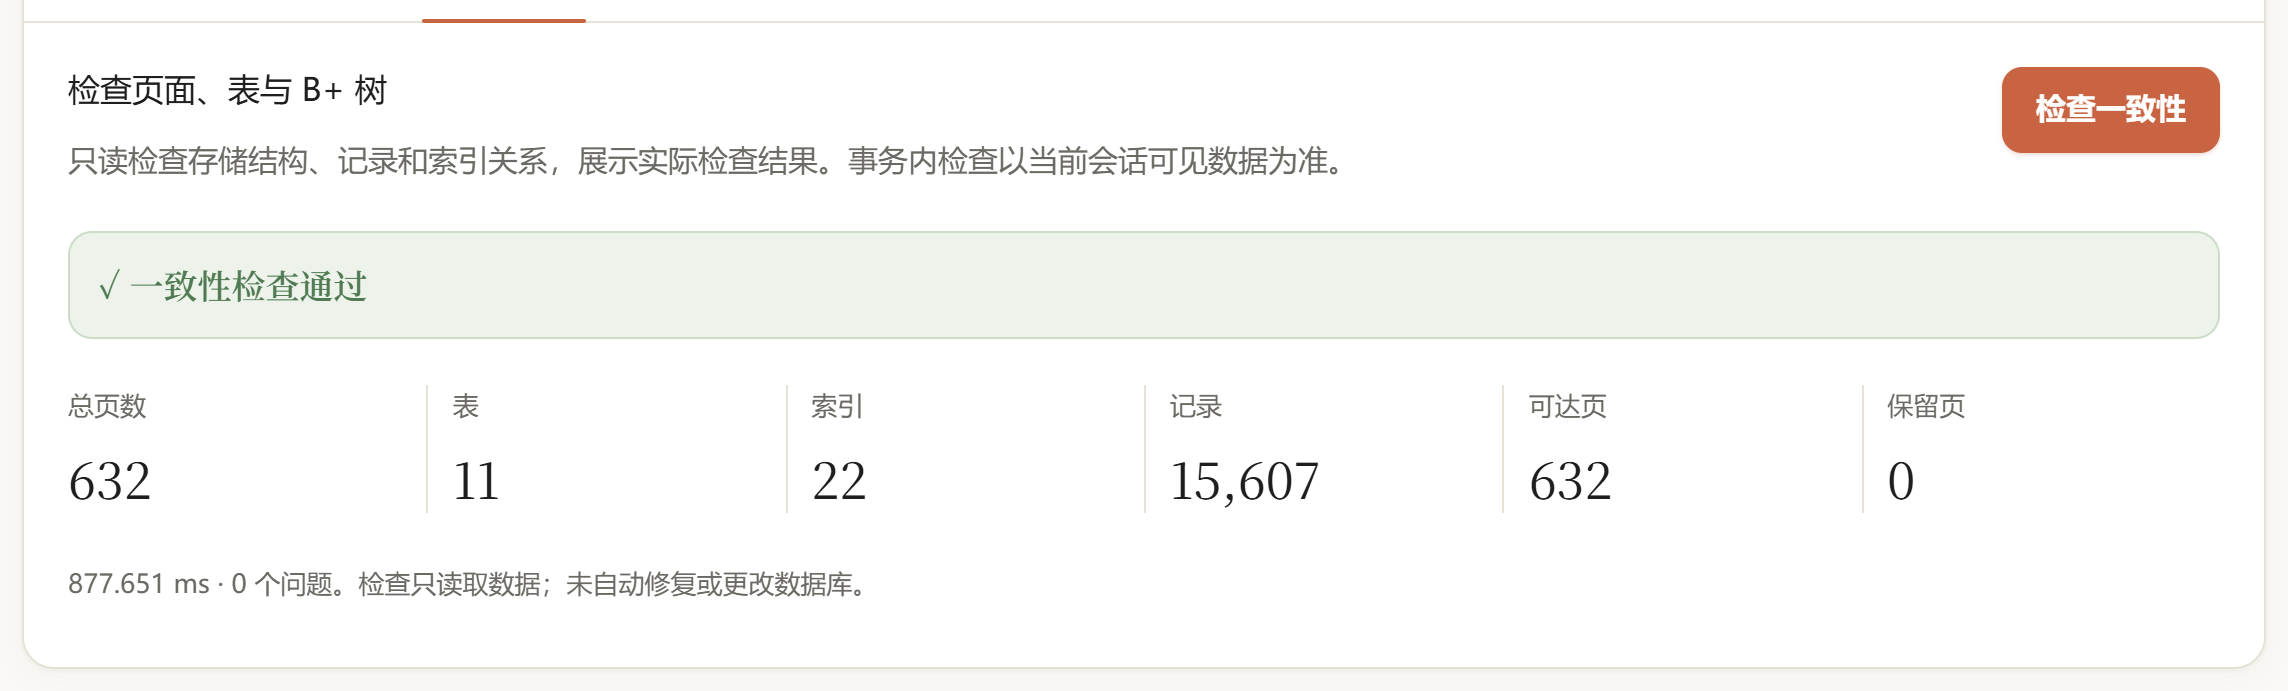
\includegraphics[width=0.92\textwidth]{fig/ui_integrity.png}
\caption{工作台“一致性检查”面板（Chinook 数据库）}\label{fig:integrity}
\end{figure}

%==================== 5 缓冲管理器 ====================
\section{缓冲管理器}\label{sec:buffer}

\subsection{已提交页缓存与事务暂存}
缓冲管理器（\fn{DiskPager}）区分两类内存页：
\begin{itemize}
  \item \textbf{已提交页缓存}：由 \fn{OrderedDict} 实现的有界 LRU，默认 64 页（256\,KiB）。命中时移到最近使用端，
        超过容量时淘汰最久未使用的页。读出和写回都复制页对象，避免调用者直接修改缓存中的字典而绕过写路径。
  \item \textbf{事务暂存页}：事务中修改过的页保存在独立的 \fn{_staged} 字典中。读页时优先返回暂存版本，
        实现“读到自己的写”；暂存页永远不会因为 LRU 淘汰而提前写入数据文件（NO-STEAL）。
        回滚时直接丢弃暂存页并恢复新页分配边界。
\end{itemize}
工作台顶部实时显示缓冲区命中率、已用缓存页数、实际读页与写页次数（见图 \ref{fig:workbench}），
它们统计的是应用层页读写，不等同于操作系统的设备 I/O。

\subsection{扫描感知的预测式淘汰}
LRU 的典型弱点是“扫描污染”：一次大范围扫描会把频繁访问的热点页全部挤出缓存。
借鉴文献 \cite{khalaji2025}，曾子恒实现了可切换的预测策略（\fn{set_buffer_policy('predictive', sample_size=8)}）：
\begin{enumerate}
  \item 堆表和 B+ 树扫描向缓冲管理器登记扫描上下文，并提供“下一页”提示；扫描结束时在 \fn{finally} 中注销。
  \item 需要淘汰时，只从少量驻留页样本中挑选候选（样本数受 \fn{sample_size} 与缓存大小限制），
        综合受限的访问频率、近期性和扫描信息，优先淘汰已被扫描越过、短期内不会再用的页，保护热点页。
  \item \textbf{扫描准入}：缓存已满、新读入的页只属于扫描、驻留页有更强的点访问历史、且没有活动扫描需要该页时，
        新页直接交给调用者而不进入缓存，避免污染。
  \item 证据不足时回退到 LRU。默认策略仍是 LRU，可随时切换回来。
\end{enumerate}
策略只作用于已提交页，不影响事务暂存与 WAL 流程；预测淘汰次数、采样次数、回退次数和准入拒绝次数都单独计数。
第 \ref{sec:exp-buffer} 节给出与同版 LRU 的对照实验。

%==================== 6 查询处理器 ====================
\section{查询处理器}\label{sec:qp}

查询处理器负责把 SQL 文本编译为可执行的计划。支持的 SQL 子集包括：
CREATE / DROP TABLE 与 INDEX（含 UNIQUE）；INTEGER、REAL、TEXT、BOOLEAN 四种类型及常用别名；
单列 PRIMARY KEY、UNIQUE、NOT NULL 与常量 DEFAULT；多行 INSERT、UPDATE、DELETE；
SELECT、DISTINCT、WHERE、INNER / LEFT / CROSS JOIN 与逗号连接、GROUP BY、HAVING、ORDER BY、LIMIT / OFFSET；
算术、比较、AND / OR / NOT、IN、BETWEEN、IS NULL、LIKE；COUNT、SUM、AVG、MIN、MAX 等聚合与常用标量函数；
BEGIN / COMMIT / ROLLBACK、CHECKPOINT、CHECK DATABASE、EXPLAIN 与 EXPLAIN ANALYZE。
子查询、窗口函数、RIGHT / FULL JOIN、外键、视图与触发器不在支持范围内，遇到时明确报错。

\subsection{词法分析}
\fn{sql.py} 中的 \fn{tokenize} 把 SQL 文本切分为关键字、标识符、数字、字符串和运算符记号，每个记号记录行号与列号，
因此任何报错都能指出具体位置。词法层处理分号分隔的多语句脚本、转义引号、双引号或反引号标识符、行注释和可嵌套的块注释；
标识符统一转为小写。

\subsection{递归下降语法分析}
语法分析器 \fn{_Parser} 为每个运算优先级编写一个函数，优先级从低到高依次为
OR、AND、NOT、比较（含 IN、BETWEEN、LIKE、IS NULL）、加减、乘除取模、一元运算和基本表达式。
例如 \texttt{a = 1 OR b = 2 AND c = 3} 会被解析为 \texttt{a = 1 OR (b = 2 AND c = 3)}。
输出的语法树由普通的字典和列表组成，例如一个 OR 节点是 \texttt{kind} 为 \texttt{binary}、\texttt{op} 为 \texttt{OR}、
带 \texttt{left} 与 \texttt{right} 两个子节点的字典；语法树只是数据，不会被当作代码执行。语法树深度限制为 128 层，防止恶意的深层括号导致 Python 递归溢出，超限时返回普通的语法错误。

\subsection{名称绑定与类型检查}
\fn{_bind} 把语法树中的列名解析为“表别名.列名”的完全限定形式，检查列是否存在、是否有歧义，
推断表达式类型并在执行前拒绝不兼容的比较；GROUP BY 查询会严格检查非聚合列。
绑定失败时给出带位置的中文错误信息，执行器不会接触到未绑定的名称。

\subsection{访问路径选择}\label{sec:scan-choice}
对每个基表，\fn{_scan_choice} 决定使用全表扫描（TableScan）还是索引扫描（IndexScan）：
\begin{enumerate}
  \item 把 WHERE 按顶层 AND 拆成若干合取项。
  \item 只有两种形状的合取项可以使用索引：\textbf{列 比较符 常量}（\texttt{= < <= > >=}）和 \textbf{列 IN (常量, …)}。
  \item 对每个可用索引的合取项，在 B+ 树中查出候选 RID，选择候选最少的那个。
  \item 启发式模式下，候选数不超过全表的 35\%（\fn{len(rids) <= max(1, total * .35)}）才走索引，
        否则离散的回表读取不如一次顺序扫描划算；自适应模式下由代价模型比较两条路径（第 \ref{sec:learning} 节）。
  \item 无论选择哪条路径，读出的行都会再用完整的 WHERE 过滤一遍，保证结果正确。
\end{enumerate}
这一设计对 AND 天然正确：任何一个合取项查出的候选都包含最终答案。但对 OR 不成立——只查 OR 的一边会漏掉满足另一边的行，
所以规划器不处理 OR 节点，\texttt{GenreId = 2 OR GenreId = 6} 只能全表扫描。这正是第 \ref{sec:trusted} 节可信改写的出发点。

\subsection{连接规划}\label{sec:join}
黄俊植负责的连接优化包含规范化、安全过滤、算法选择与有界顺序搜索。
\begin{itemize}
  \item \textbf{规范化与过滤}：名称绑定后，\fn{join_planning.py} 将纯内连接的逗号、CROSS JOIN 与 ON / WHERE 条件统一组织，
        只拆分顶层 AND；跨表条件归入最早可计算的连接前缀。LEFT JOIN 保持顺序，可空侧 WHERE 条件仍在补空后检查。
  \item \textbf{物理算法}：等值条件优先使用哈希连接；自适应模式可对直接列的范围条件排序右输入、二分定位候选，
        再检查完整 ON；其余条件保留嵌套循环。
\end{itemize}

\paragraph{状态与递推} \fn{choose_inner_join_order()} 按表集合自底向上构造左深计划。状态记录表集合、顺序、预计行数、
累计成本与置信度；从各单表起点出发，每次沿已有连接边加入一张表，累计：
\begin{equation*}
C_{\text{new}} = C_{\text{prefix}} + C_{\text{access}} + C_{\text{join}}.
\end{equation*}

\paragraph{候选复用与剪枝} 同一表集合保留多个各有优势的候选。若一个前缀成本不高、行数不多、置信度不低且至少一项更优，
则淘汰被其支配者；当前较便宜但行数更多的前缀仍可能保留，因为输出规模影响后续成本。

\paragraph{预算与回退} 自适应模式在统计可用时搜索 3--6 表连通等值内连接，限 512 个扩展前缀和约 20\,ms 协作预算（非硬时限）。
模型未就绪或域外时仍可用统计与规则成本搜索；统计不足、形状不支持、预算耗尽或置信度 / 收益不足时才保留原顺序。
执行一个计划，不保证全局最优。

\subsection{统计信息与学习型代价模型}\label{sec:learning}
\fn{Database.analyze_statistics()} 只读扫描已提交堆表，采集行数、NULL 数、不同值数量（NDV）、取值范围、
最多 12 桶直方图和 24 个高频值。统计先给出过滤与等值连接规模初值，模型再利用执行反馈校准；模型不直接生成查询结果。

\paragraph{四类模型及其输入、目标与用途} \fn{learning.py} 使用通用的 \fn{RidgeModel(width)}，维度包含截距特征 1，
按任务配置为 2、3 或 4 维。扫描和索引读取分别建模，过滤和连接校准按相应条件或表列关系保存模型实例。

\begin{table}[H]
\centering\small
\caption{学习型代价模型}\label{tab:models}
\begin{tabularx}{\textwidth}{>{\raggedright}p{2.0cm}>{\raggedright}X>{\raggedright}p{2.6cm}>{\raggedright\arraybackslash}p{4.0cm}}
\toprule
\textbf{模型 / 维度} & \textbf{输入特征} & \textbf{实际训练目标} & \textbf{预测用途} \\
\midrule
过滤校准\newline 2 维 & $[1, s_{\text{stat}}]$，其中 $s_{\text{stat}}$ 为统计选择率 & 通过行数 / 表行数 & 校准比例乘总行数，得到预计过滤行数 \\
等值连接\newline 校准 / 4 维 & 原始连接选择率、两侧相对原表规模，以及截距 1 & 连接输出 / 两侧输入行数乘积 & 校准比例乘输入乘积，得到预计连接行数 \\
读取成本\newline 3 维 & $[1, N/1000, P/100]$；$N$ 为读取行数，$P$ 为页数 & 扫描或索引读取耗时（ms） & 比较两条读路径；预测差异不足时仍用规则选择 \\
哈希连接\newline 成本 / 4 维 & $[1, L/1000, R/1000, O/1000]$；$L, R, O$ 为两侧输入及输出行数 & 实际哈希连接算子耗时（ms） & 累计到候选计划成本，帮助比较连接顺序 \\
\bottomrule
\end{tabularx}
\end{table}

\paragraph{统计初估与模型校准} 等值连接的初值按输入规模、NDV 与非空比例计算，并采用均匀性等假设；单表 AND 条件可按独立性组合，
受支持的单个条件才直接使用过滤校准模型。例如统计选择率为 1\% 时，过滤模型输入为 $[1, 0.01]$，由训练得到的权重计算校准比例，
再乘表行数；输入特征不是权重。校准比例限制在 0 到 1 之间。

\paragraph{岭回归与轻量实现} 岭回归最小化预测误差平方和并对权重加正则项：
\begin{equation*}
\min_{w} \sum_i \bigl(y_i - w^{\mathsf T} x_i\bigr)^2 + \sum_j \lambda_j w_j^2 .
\end{equation*}
\fn{RidgeModel.observe()} 形成小型正则化正规方程，由 \fn{_solve()} 求解；\fn{predict()} 计算预测值。
低维线性模型的训练与预测开销小，权重正则可缓解小样本拟合的不稳定性。连接耗时模型针对哈希连接，不混入范围连接的排序耗时。

\paragraph{执行反馈闭环} 统计管理、估计学习、计划选择与执行反馈形成闭环。普通查询只执行一个选定计划，不逐一试跑候选连接；
规划期间仍可能查询索引取得候选 RID。

执行器反馈实际通过 / 连接比例、读取与哈希连接耗时。读成本样本使用应用缓冲池冷状态，保留操作系统缓存。
计划记录预计与实际行数、估计误差及成本来源，便于检查预测是否有效。

\paragraph{样本维护与模型适用性} 每个模型最多保留最近 96 个样本，至少有 8 个样本、3 种不同特征向量时才可能就绪。
模型检查数值有效性；校准模型不采用违反所需单调条件的系数。预测还检查非截距特征是否落在各维训练范围内，域外输入不进行任意外推；
部分模型另结合误差与收益门槛决定是否采用。这是保守的适用性检查，不是任意分布偏移下的泛化保证。

\paragraph{有界工作负载管理} \fn{workload.py} 的 \fn{WorkloadManager} 按语法树形状和字面量类型生成查询指纹，
最多保存 128 类查询的聚合反馈。记录包括执行次数、平均耗时、读页、扫描行数、连接候选比较、估计误差，
以及最近的访问路径和连接顺序；该管理器不保存 SQL 字面量值或结果行。

数据代次、统计代次和模型版本兼容时，历史顺序通过 \fn{preferred_order()} 参与近似同价候选的稳定性选择。
它不替代动态规划，不跳过搜索，也不等同于完整计划或查询结果缓存。

\paragraph{版本失效与重新学习} 写入、事务状态变化和重新采集统计会保守地使旧统计、模型与相关结论失效。
\fn{ResearchState.invalidate()} 清理旧状态并更新代次；重新采集统计后发布新摘要。缓冲配置切换通过
\fn{reset_buffer_learning()} 保留列统计，但清除读成本等学习模型、工作负载反馈与相关结论，避免继续使用旧环境下的经验。

\paragraph{分层回退与正确性} 过滤或等值连接校准不可用时，回到统计初估及其边界处理；操作成本模型不可用时，回到规则成本。
只有计划搜索本身条件不满足时，才保留原 SQL 连接顺序；“模型未就绪”不等于“查询不能优化”。
默认 heuristic 模式仍提供规则对照。模型只影响计划选择，真实查询结果由确定性执行器计算。

%==================== 7 执行引擎 ====================
\section{执行引擎}\label{sec:executor}

\subsection{算子与物化执行}
执行引擎把计划组织为一棵算子树，表 \ref{tab:ops} 列出主要算子。执行采用\textbf{物化}方式 \cite{graefe1993}：
每个算子把结果全部算完后再整体交给上层。这种方式实现简单、每一步处理的行数容易统计，代价是中间结果较大时占用内存，
因此执行器对扫描行数、连接比较次数和中间结果规模设置了协作式预算。

\begin{table}[!htb]
\centering\small
\caption{执行引擎的主要算子}\label{tab:ops}
\begin{tabularx}{\textwidth}{>{\ttfamily}p{3.3cm}X}
\toprule
\normalfont 算子 & 作用 \\
\midrule
TableScan & 按堆页顺序读出整张表 \\
IndexScan & 按 B+ 树给出的 RID 回表读取 \\
Filter & 按 WHERE 条件过滤（可下推到基表扫描） \\
HashJoin & 等值连接：对一侧输入按连接键建哈希表，另一侧逐行探测 \\
RangeJoin & 范围连接：排序 + 二分定位候选区间 \\
NestedLoopJoin & 其他连接条件的通用实现 \\
HashAggregate & GROUP BY 分组与 COUNT / SUM / AVG / MIN / MAX \\
Project / Distinct & 计算输出列；按带类型的键去重 \\
Sort / Limit & 排序（NULL 升序在前、降序在后）；分页 \\
\bottomrule
\end{tabularx}
\end{table}

图 \ref{fig:plan} 是 Chinook 上“曲目最多的前 10 位艺术家”查询的执行计划。读法是缩进越深越先执行：
三张表各扫描一次（275 + 347 + 3\,503 = 4\,125 行，即工作台显示的扫描行数），两次哈希连接把曲目与专辑、艺术家拼接，
再按艺术家分组计数、排序并取前 10 行。图中的行数是规划器在执行前的估计值，实际值以 EXPLAIN ANALYZE 为准。

\begin{figure}[!htb]
\centering
\begin{tikzpicture}[every node/.style={font=\small}, level distance=9mm]
  \tikzset{op/.style={draw=accent, fill=soft, rounded corners=2pt, inner sep=3pt, align=left,
                      font=\small\ttfamily, anchor=west}}
  \node[op] (l) at (0,0) {Limit \normalfont\footnotesize（10 行）};
  \node[op] (s) at (0.7,-0.85) {Sort \normalfont\footnotesize tracks DESC, artist};
  \node[op] (p) at (1.4,-1.7) {Project \normalfont\footnotesize artist, tracks};
  \node[op] (a) at (2.1,-2.55) {HashAggregate \normalfont\footnotesize 按 ar.name 分组};
  \node[op] (j1) at (2.8,-3.4) {HashJoin \normalfont\footnotesize al.albumid = tr.albumid（估计 3\,503 行）};
  \node[op] (j2) at (3.5,-4.25) {HashJoin \normalfont\footnotesize ar.artistid = al.artistid（估计 347 行）};
  \node[op] (t1) at (4.2,-5.1) {TableScan artist \normalfont\footnotesize（275 行）};
  \node[op] (t2) at (4.2,-5.95) {TableScan album \normalfont\footnotesize（347 行）};
  \node[op] (t3) at (3.5,-6.8) {TableScan track \normalfont\footnotesize（3\,503 行）};
  \foreach \u/\v in {l/s,s/p,p/a,a/j1,j1/j2,j2/t1,j2/t2,j1/t3}{
    \draw[black!45] ([xshift=3mm]\u.south west) |- (\v.west);}
\end{tikzpicture}
\caption{Chinook 三表连接聚合查询的执行计划树}\label{fig:plan}
\end{figure}

\subsection{NULL 语义与类型规则}
表达式求值遵循 SQL 的三值逻辑：比较中任一侧为 NULL 时结果为“未知”，\texttt{sql\_and} / \texttt{sql\_or} 按真值表合成，
WHERE 只保留结果为“真”的行。除法返回实数、除以零返回 NULL；DISTINCT 与 GROUP BY 使用带类型的键，
BOOLEAN 不与数值 0 / 1 合并；连接在选择物理算法之前先校验比较类型，避免哈希连接与嵌套循环在类型不兼容时给出不同结果。

\subsection{事务}
默认自动提交，每条语句是一个事务。\texttt{BEGIN} 之后的修改只进入暂存页，其他查询看不到；
\texttt{COMMIT} 按第 \ref{sec:storage} 节的流程持久化；\texttt{ROLLBACK} 丢弃暂存页。
显式事务中任何一条语句出错，整个事务回滚，不会出现部分生效。系统是单写者设计，不提供并发事务与 MVCC。

\subsection{EXPLAIN 与执行计数}
\texttt{EXPLAIN} 只生成计划不读数据；\texttt{EXPLAIN ANALYZE} 真正执行查询，并在计划中附上实际行数、
扫描行数、索引查找次数、连接比较次数和耗时。工作台的“执行计划”页与“扫描对比”工具都基于这些真实计数。

%==================== 8 创新点 ====================
\section{研究扩展与创新点}\label{sec:innovation}

\subsection{可信查询改写（钟国鹏）}\label{sec:trusted}

\subsubsection{问题}
查询改写是“换一种写法，意思不变，执行更快”。在第 \ref{sec:scan-choice} 节的规划器下，下面两条查询语义相同，但执行代价差别很大：
\begin{lstlisting}[style=sql]
-- original: TableScan, 3503 rows
SELECT TrackId, Name, Milliseconds FROM Track WHERE GenreId = 2 OR GenreId = 6;
-- rewritten: IndexScan, 211 rows
SELECT TrackId, Name, Milliseconds FROM Track WHERE GenreId IN (2, 6);
\end{lstlisting}
改写的风险在于“改错了，结果就错了”。一般 SQL 的等价性不可判定 \cite{chu2017}，而“在当前数据上结果相同”只是等价的必要条件：
例如候选 \texttt{GenreId IN (6, 2) AND Milliseconds >= 0} 在现有数据上与原查询结果完全一样，
但只要插入一条时长为负数或为 NULL 的错误数据，候选就会少返回一行。
由 LLM 生成的改写同样没有等价保证 \cite{narasayya2026,resequel2026}。因此我们需要一个机制，
\textbf{只接受能证明没改错、全量结果一致且确实更快的改写，其余一律保留原查询}。

\subsubsection{可信规则}
\fn{optimizer.py} 中的 \fn{trusted_rewrite} 只对 WHERE 子句应用三条手写规则，投影、分组、排序和连接结构不变：
\begin{itemize}
  \item \fn{or-equalities-to-in}：同一列上 2--32 个“列 = 常量”用 OR 连接时合并为 IN。前置条件为：每一项都是等值比较、
        一侧是同一个列、另一侧是常量，且常量类型与列类型匹配（避免隐式类型转换带来的差异）；任一条件不满足即原样返回。
  \item \fn{duplicate-and}：删除 AND 中完全相同的合取项。
  \item \fn{where-true}：删除恒为真的条件。
\end{itemize}
以 OR→IN 为例，WHERE 对每一行独立求值，一行的 GenreId 只有表 \ref{tab:truth} 中四种情况，两种写法的真值在每种情况下都相同，
因此在任何数据上都选出完全相同的行（WHERE 只决定行的去留，不改变重复次数）。

\begin{table}[!htb]
\centering\small
\caption{OR→IN 改写的逐行真值对照（含 NULL）}\label{tab:truth}
\begin{tabular}{cccc}
\toprule
该行 GenreId & \texttt{GenreId = 2 OR GenreId = 6} & \texttt{GenreId IN (2, 6)} & 该行 \\
\midrule
2 & 真 OR 假 = 真 & 真 & 两边都保留 \\
6 & 假 OR 真 = 真 & 真 & 两边都保留 \\
其他值 & 假 OR 假 = 假 & 假 & 两边都丢弃 \\
NULL & 未知 OR 未知 = 未知 & 未知 & 两边都丢弃 \\
\bottomrule
\end{tabular}
\end{table}

\subsubsection{三道关卡}
\fn{optimize(db, sql, candidate_sql=None)} 实现图 \ref{fig:gates} 的闭环。候选可以由本地规则生成，也可以由用户手写或由大模型给出，
系统对所有来源一视同仁地检查。实验在执行前还会拒绝带 LIMIT / OFFSET 的候选以及 ORDER BY 不一致的候选。

\begin{figure}[!htb]
\centering
\begin{tikzpicture}[node distance=11mm]
  \node[plain, text width=3.0cm] (c) {候选改写\\{\footnotesize 本地规则 / 手写 / 大模型}};
  \node[box, below=of c, text width=3.0cm] (g1) {关卡 1 · 规则证据};
  \node[box, below=of g1, text width=3.0cm] (g2) {关卡 2 · 结果核验};
  \node[box, below=of g2, text width=3.0cm] (g3) {关卡 3 · 收益门槛};
  \node[plain, below=of g3, text width=3.0cm, draw=okgreen, fill=okgreen!8] (ok) {建议替换（proven）\\{\footnotesize 用户点击“填入编辑器”才生效}};
  \draw[arr] (c)--(g1); \draw[arr] (g1)--(g2); \draw[arr] (g2)--(g3); \draw[arr] (g3)--(ok);
  \node[note, right=6mm of g1, text width=7.2cm] {候选与“规则从原查询推导出的结果”语法树逐字相同 → 暂定 proven，记录规则名与两棵树的 SHA-256；否则最高只能是 tested};
  \node[note, right=6mm of g2, text width=7.2cm] {两条查询在全部数据上各执行一次，按\textbf{多重集合}比较结果（区分重复行、NULL 与类型）；不一致 → unknown，拒绝};
  \node[note, right=6mm of g3, text width=7.2cm] {各跑 3 次、每次前清空缓存，取中位数与 MAD；收益须超过 $\max(1\,\mathrm{ms},\ 15\%,\ 3\times\text{噪声})$，且原查询 $\ge 2$ ms；否则保留原查询};
\end{tikzpicture}
\caption{可信改写的三道关卡}\label{fig:gates}
\end{figure}

收益门槛的完整定义为（\fn{optimizer.py}）：
\begin{gather}
\text{margin} = \max\bigl(1.0,\ 0.15\,t_{\text{orig}},\ 3(\text{MAD}_{\text{orig}}+\text{MAD}_{\text{cand}})\bigr),\\
\text{replace} = (t_{\text{orig}} \ge 2.0)\ \wedge\ (t_{\text{orig}} - t_{\text{cand}} \ge \text{margin}),
\end{gather}
其中 $t$ 为 3 次冷缓存执行耗时的中位数（毫秒）。原查询本身很快时，验证的开销超过可能的收益，系统选择不替换，
这一点借鉴了 ReSequel 把验证成本计入收益的思想 \cite{resequel2026}。
结论分为三级：\textbf{proven}（规则可推导且结果一致）、\textbf{tested}（只是当前数据上一致，不建议自动替换）、
\textbf{unknown}（结果不同或无法比较）。全过程只执行 SELECT，不修改任何数据。

“已证明”的含义是：候选由经过审查的规则推导而来，推导过程可以重放检查。它不是通用的等价证明器——那在理论上不存在。
这一“证明不了就如实说未知”的分级思想借鉴自文献 \cite{narasayya2026}。

\subsubsection{演示结果}
图 \ref{fig:rewrite} 是在 Chinook 上对上述 OR 查询运行可信改写的结果：三道关卡全部通过，
扫描行数由 3\,503 降为 211，文件读页由 158 降为 28，查询耗时由 75.4 ms 降为 37.4 ms（2.02 倍），
收益 37.99 ms 超过门槛 16.05 ms（本次测量中三倍噪声项大于 15\% 项），因此建议替换。
各次运行的毫秒数会随机器负载波动，但扫描行数与读页数是确定的。作为对照，图 \ref{fig:compare} 的“扫描对比”工具显示，
原 OR 查询在“强制全表扫描”和“优化器选择”两条路径下都读了 3\,503 行——规划器确实无法为 OR 使用索引。

\begin{figure}[!htb]
\centering
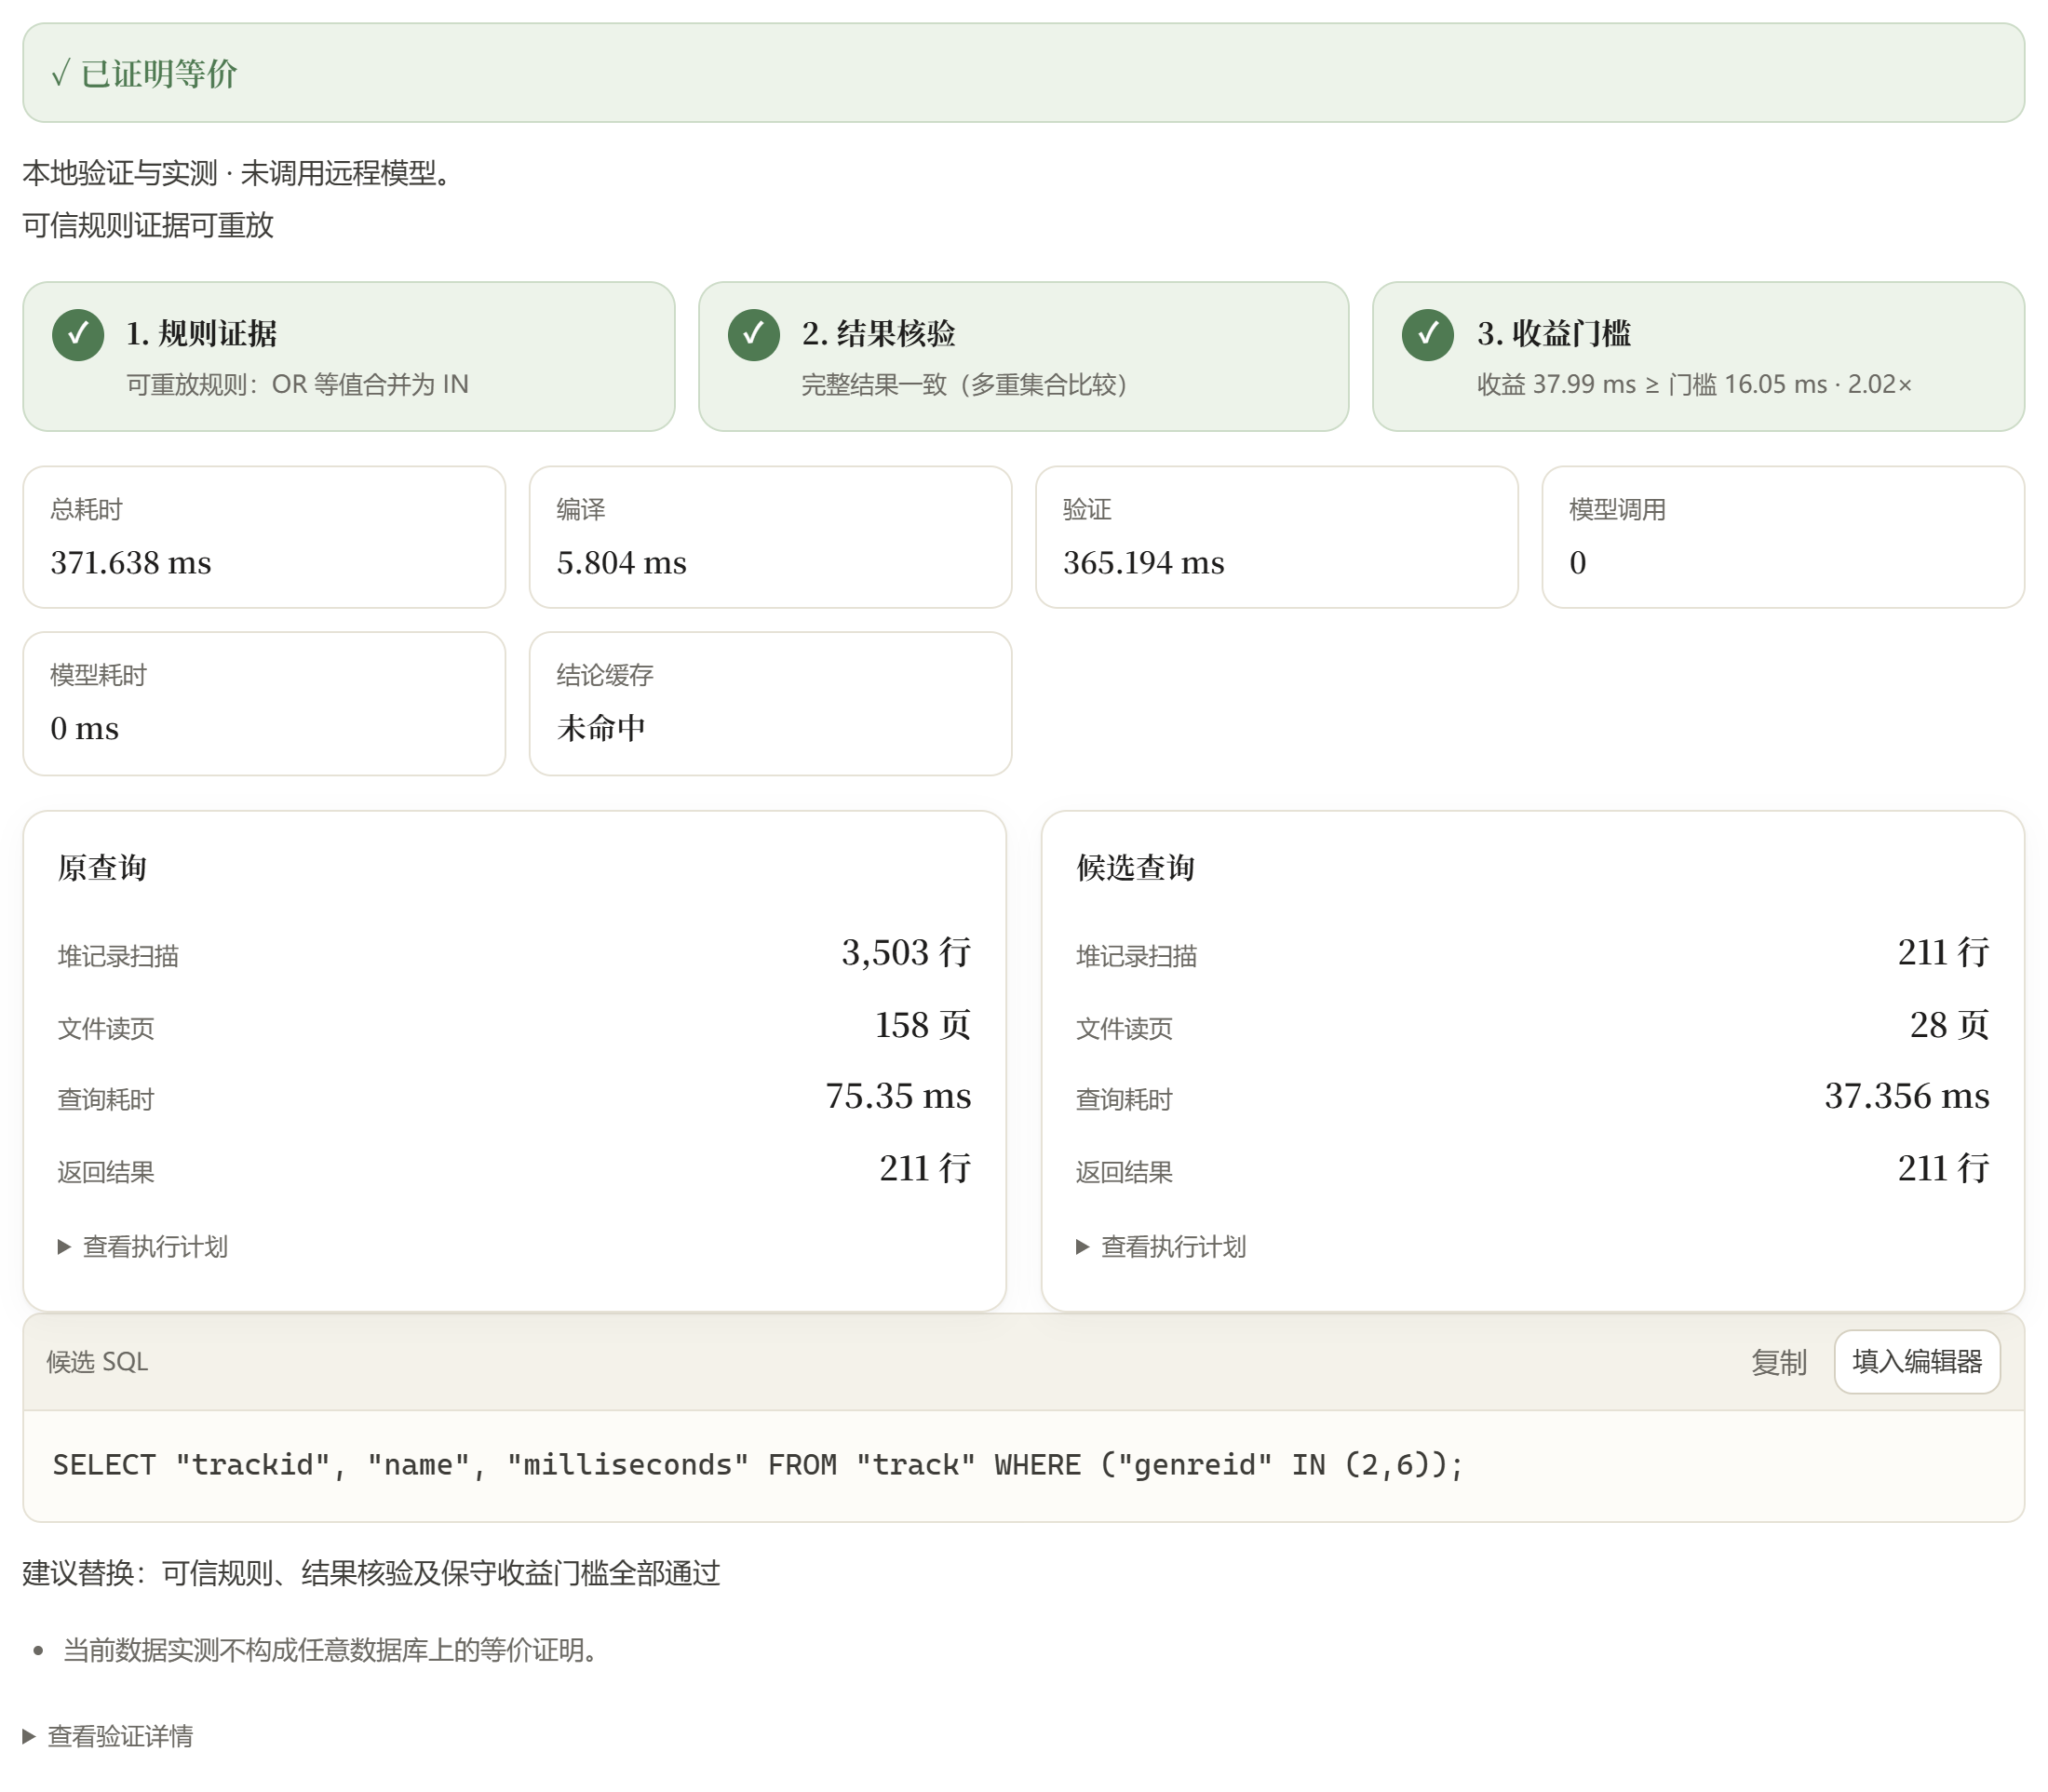
\includegraphics[width=0.84\textwidth]{fig/ui_rewrite.png}
\caption{工作台“研究实验 → 可信改写”面板：OR→IN 改写通过三道关卡}\label{fig:rewrite}
\end{figure}

\begin{figure}[!htb]
\centering
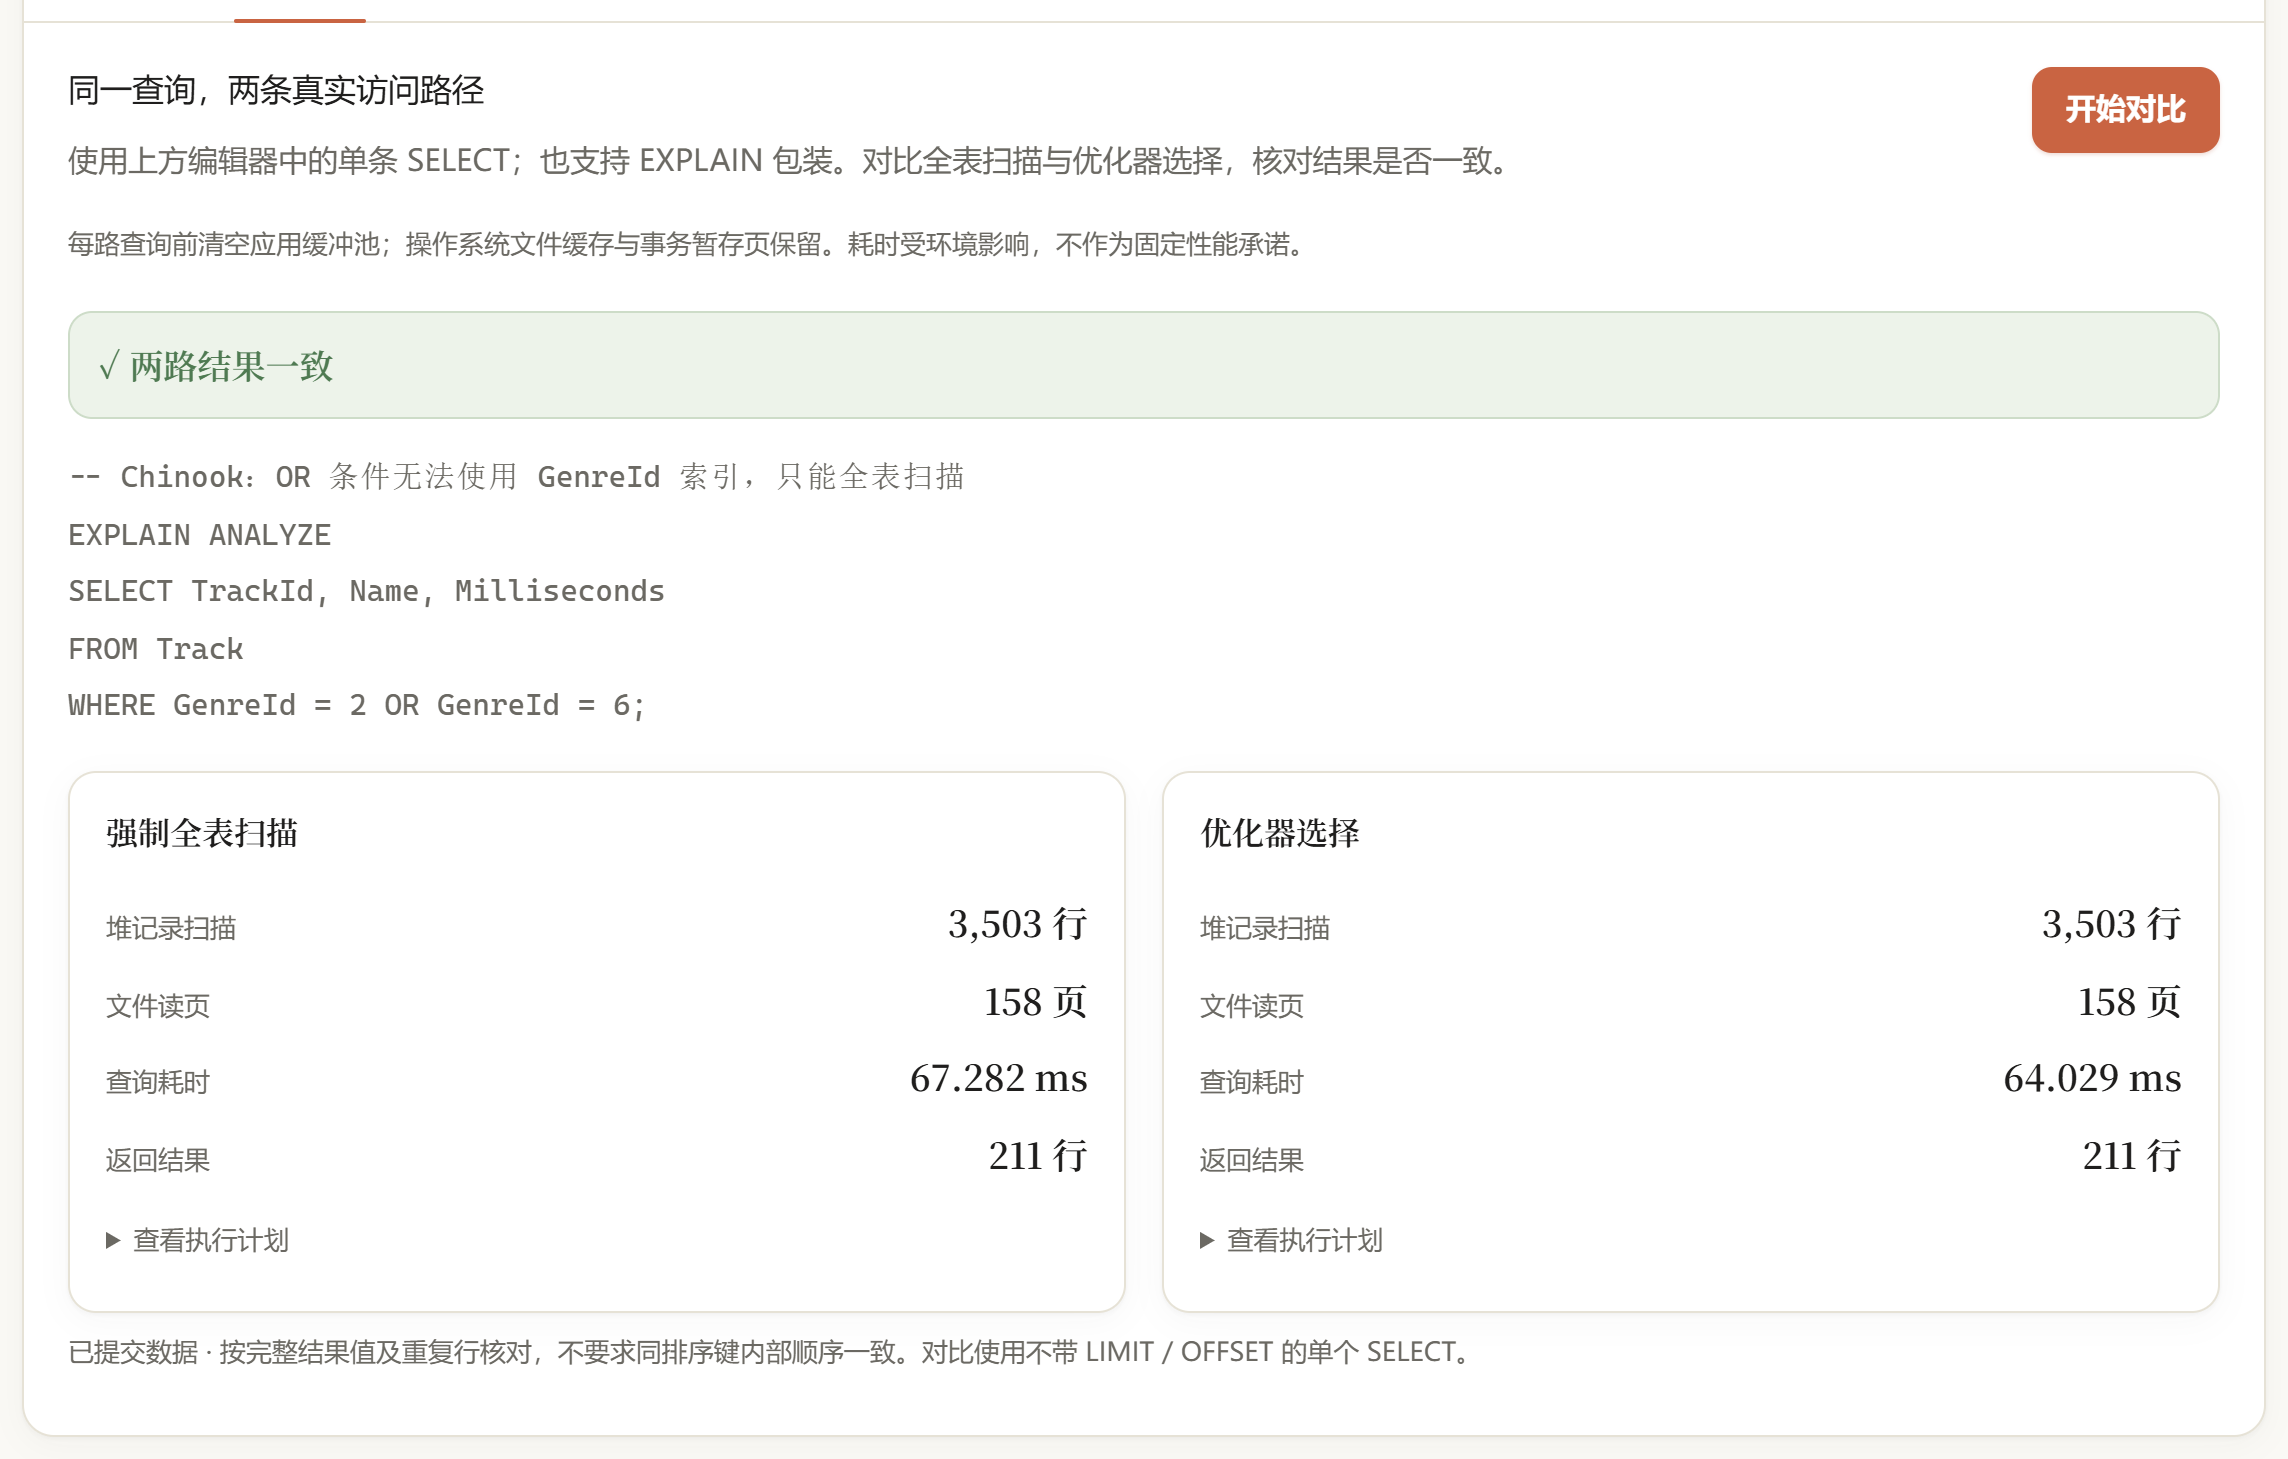
\includegraphics[width=0.84\textwidth]{fig/ui_compare.png}
\caption{“扫描对比”工具：原 OR 查询的两条访问路径都只能全表扫描}\label{fig:compare}
\end{figure}

\subsection{统计学习与自适应连接规划（黄俊植）}
该扩展把第 \ref{sec:learning} 节的统计信息与代价模型用于访问路径和连接顺序选择，目标是在训练范围内降低估计误差、
减少中间结果，在越出范围时安全回退。设计上借鉴 PRICE 的统计特征 \cite{price2024} 和 CardOOD 对分布偏移的关注 \cite{cardood2026}，
但只实现标准库中的轻量模型，不进行跨数据库预训练。

图 \ref{fig:join} 是中文教学库上的三表连接演示：按 SQL 书写顺序执行时，先连接选课与课程，产生 10\,000 行中间结果，
连接候选比较 20\,000 次；自适应规划先用 \texttt{p.department = 'CS'} 过滤学生表，再按“学生 → 选课 → 课程”的顺序连接，
中间结果只有 100 行，候选比较降为 200 次，两种执行的完整结果（含重复行）一致。

\begin{figure}[!htb]
\centering
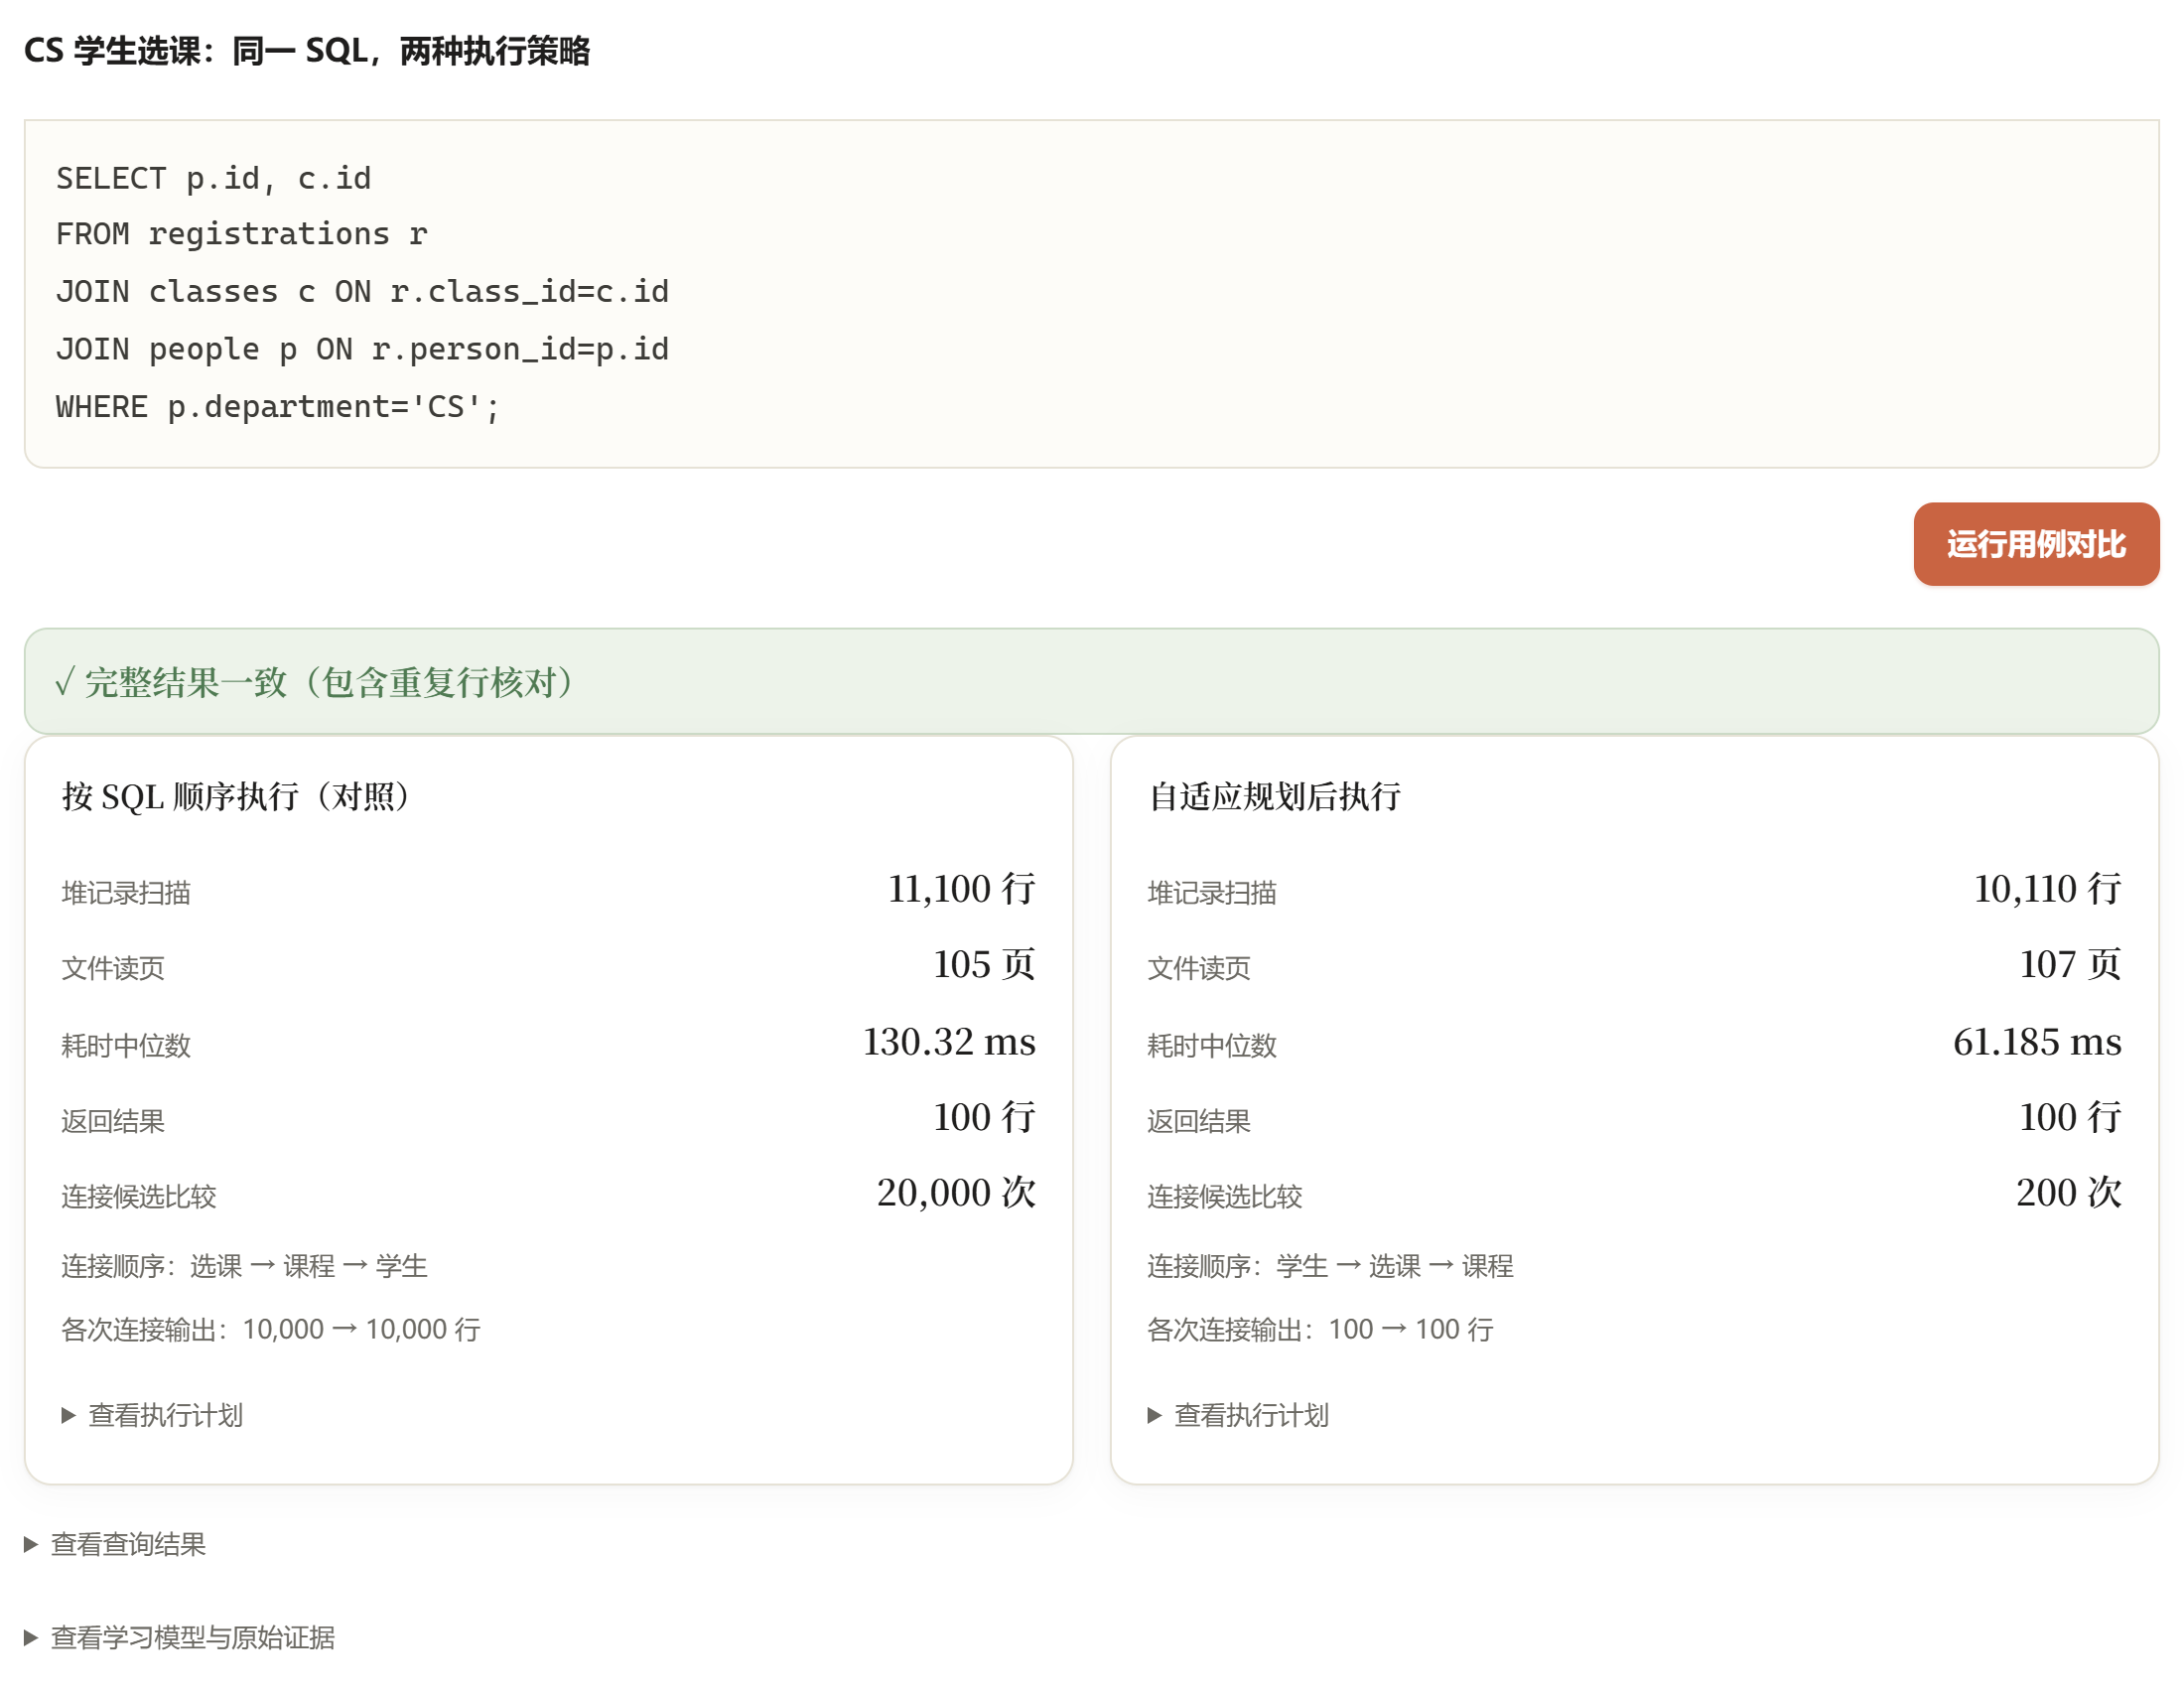
\includegraphics[width=0.80\textwidth]{fig/ui_join.png}
\caption{同一 SQL 的两种连接执行策略对比}\label{fig:join}
\end{figure}

\subsection{扫描感知的预测缓冲（曾子恒）}
预测策略的设计见第 \ref{sec:buffer} 节。它针对的是单连接串行执行中“大扫描与热点点读交替”造成的缓存污染，
以及热点迁移后频率历史的适应性。与原论文 \cite{khalaji2025} 不同，本项目没有并发长扫描，也没有在真实云数据仓库负载上评测，
因此实验收益不能视为该论文的复现结果。实验结果见第 \ref{sec:exp-buffer} 节。

\subsection{受预算约束的 AI 语义算子（路茗淳）}
借鉴 iPDB \cite{ipdb2026}，本项目把大模型的判断做成有明确输入、输出和代价的关系算子，而不是让模型直接生成并执行 SQL：
\begin{itemize}
  \item 先由确定性的 SQL 执行器物化一次 SELECT，再把用户选择的 TEXT 列交给语义管线。
        \textbf{SemanticFilter} 保留模型判为匹配的完整原行；\textbf{SemanticProject} 附加布尔判断与短标签；
        \textbf{SemanticAggregate} 对标签做确定性计数。NULL 不发送给模型。
  \item 同一次运行内先按完整文本去重，再按批调用 Chat Completions 接口；响应必须对每个输入 ID 恰好返回一个结果，
        缺失、重复、越界或类型错误都会被拒绝。精确缓存默认容量 512 条、有效期 300 秒，缓存键包含文本、条件、模型和服务配置的摘要，不保存明文凭证。
  \item 默认最多 64 行、每批 8 条、最多 8 批，SQL 与推理总预算 30 秒；推理期间不持有数据库锁，普通 SQL 可以继续执行。
  \item 未配置模型时提供“关键词：词一|词二”的本地确定性演示模式，并明确标注“未调用大模型”。
\end{itemize}
系统也已接入上海交通大学校园大模型服务（\fn{deepseek-chat}）完成小样本真实验收，验收记录保存在 \fn{docs/campus_api_smoke.json}。
图 \ref{fig:semantic} 为本地演示模式下的语义筛选结果。

\begin{figure}[!htb]
\centering
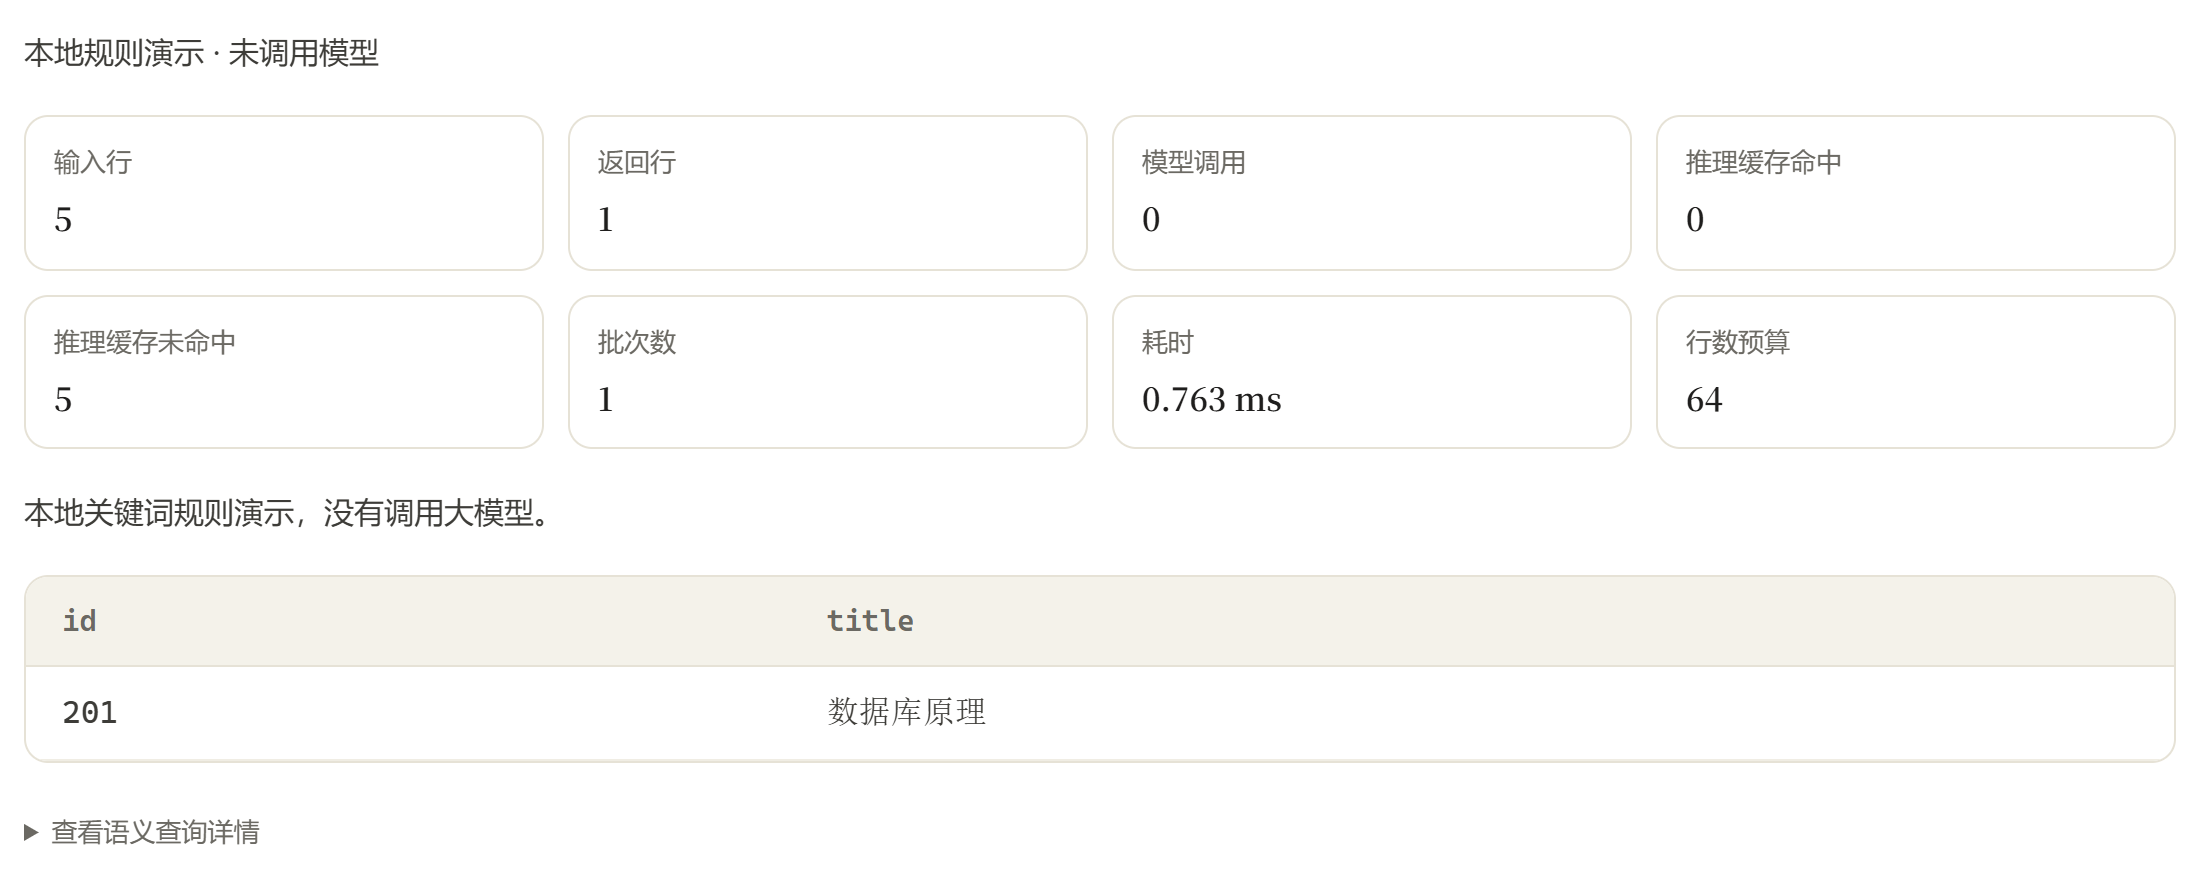
\includegraphics[width=0.80\textwidth]{fig/ui_semantic.png}
\caption{语义筛选算子：输入 5 行课程，筛出与“数据库 / 查询 / 索引”相关的 1 行（本地规则演示）}\label{fig:semantic}
\end{figure}

%==================== 9 用户界面 ====================
\section{用户界面与使用说明}\label{sec:ui}

\subsection{浏览器工作台}
工作台（图 \ref{fig:workbench}）由 \fn{server.py} 提供本机 HTTP 服务，前端为不依赖框架的 HTML / CSS / JavaScript。主要区域包括：
\begin{itemize}
  \item 左侧：数据库对象列表，显示每张表的行数，点击字段可插入 SQL；
  \item 顶部：事务状态、缓冲区命中率、缓存页、实际读页与写页次数；
  \item 中部：带语法高亮和行号的 SQL 编辑器、示例下拉菜单，\texttt{Ctrl + Enter} 执行选区或全部语句；
  \item 结果区：“查询结果”与“执行计划”两个标签页，显示行数和耗时；
  \item 工具区：AI 助手、扫描对比、一致性检查和研究实验（可信改写、优化模式、缓冲策略、语义算子）四个面板；
  \item 浅色 / 深色 / 跟随系统三种主题。
\end{itemize}

\begin{figure}[!htb]
\centering
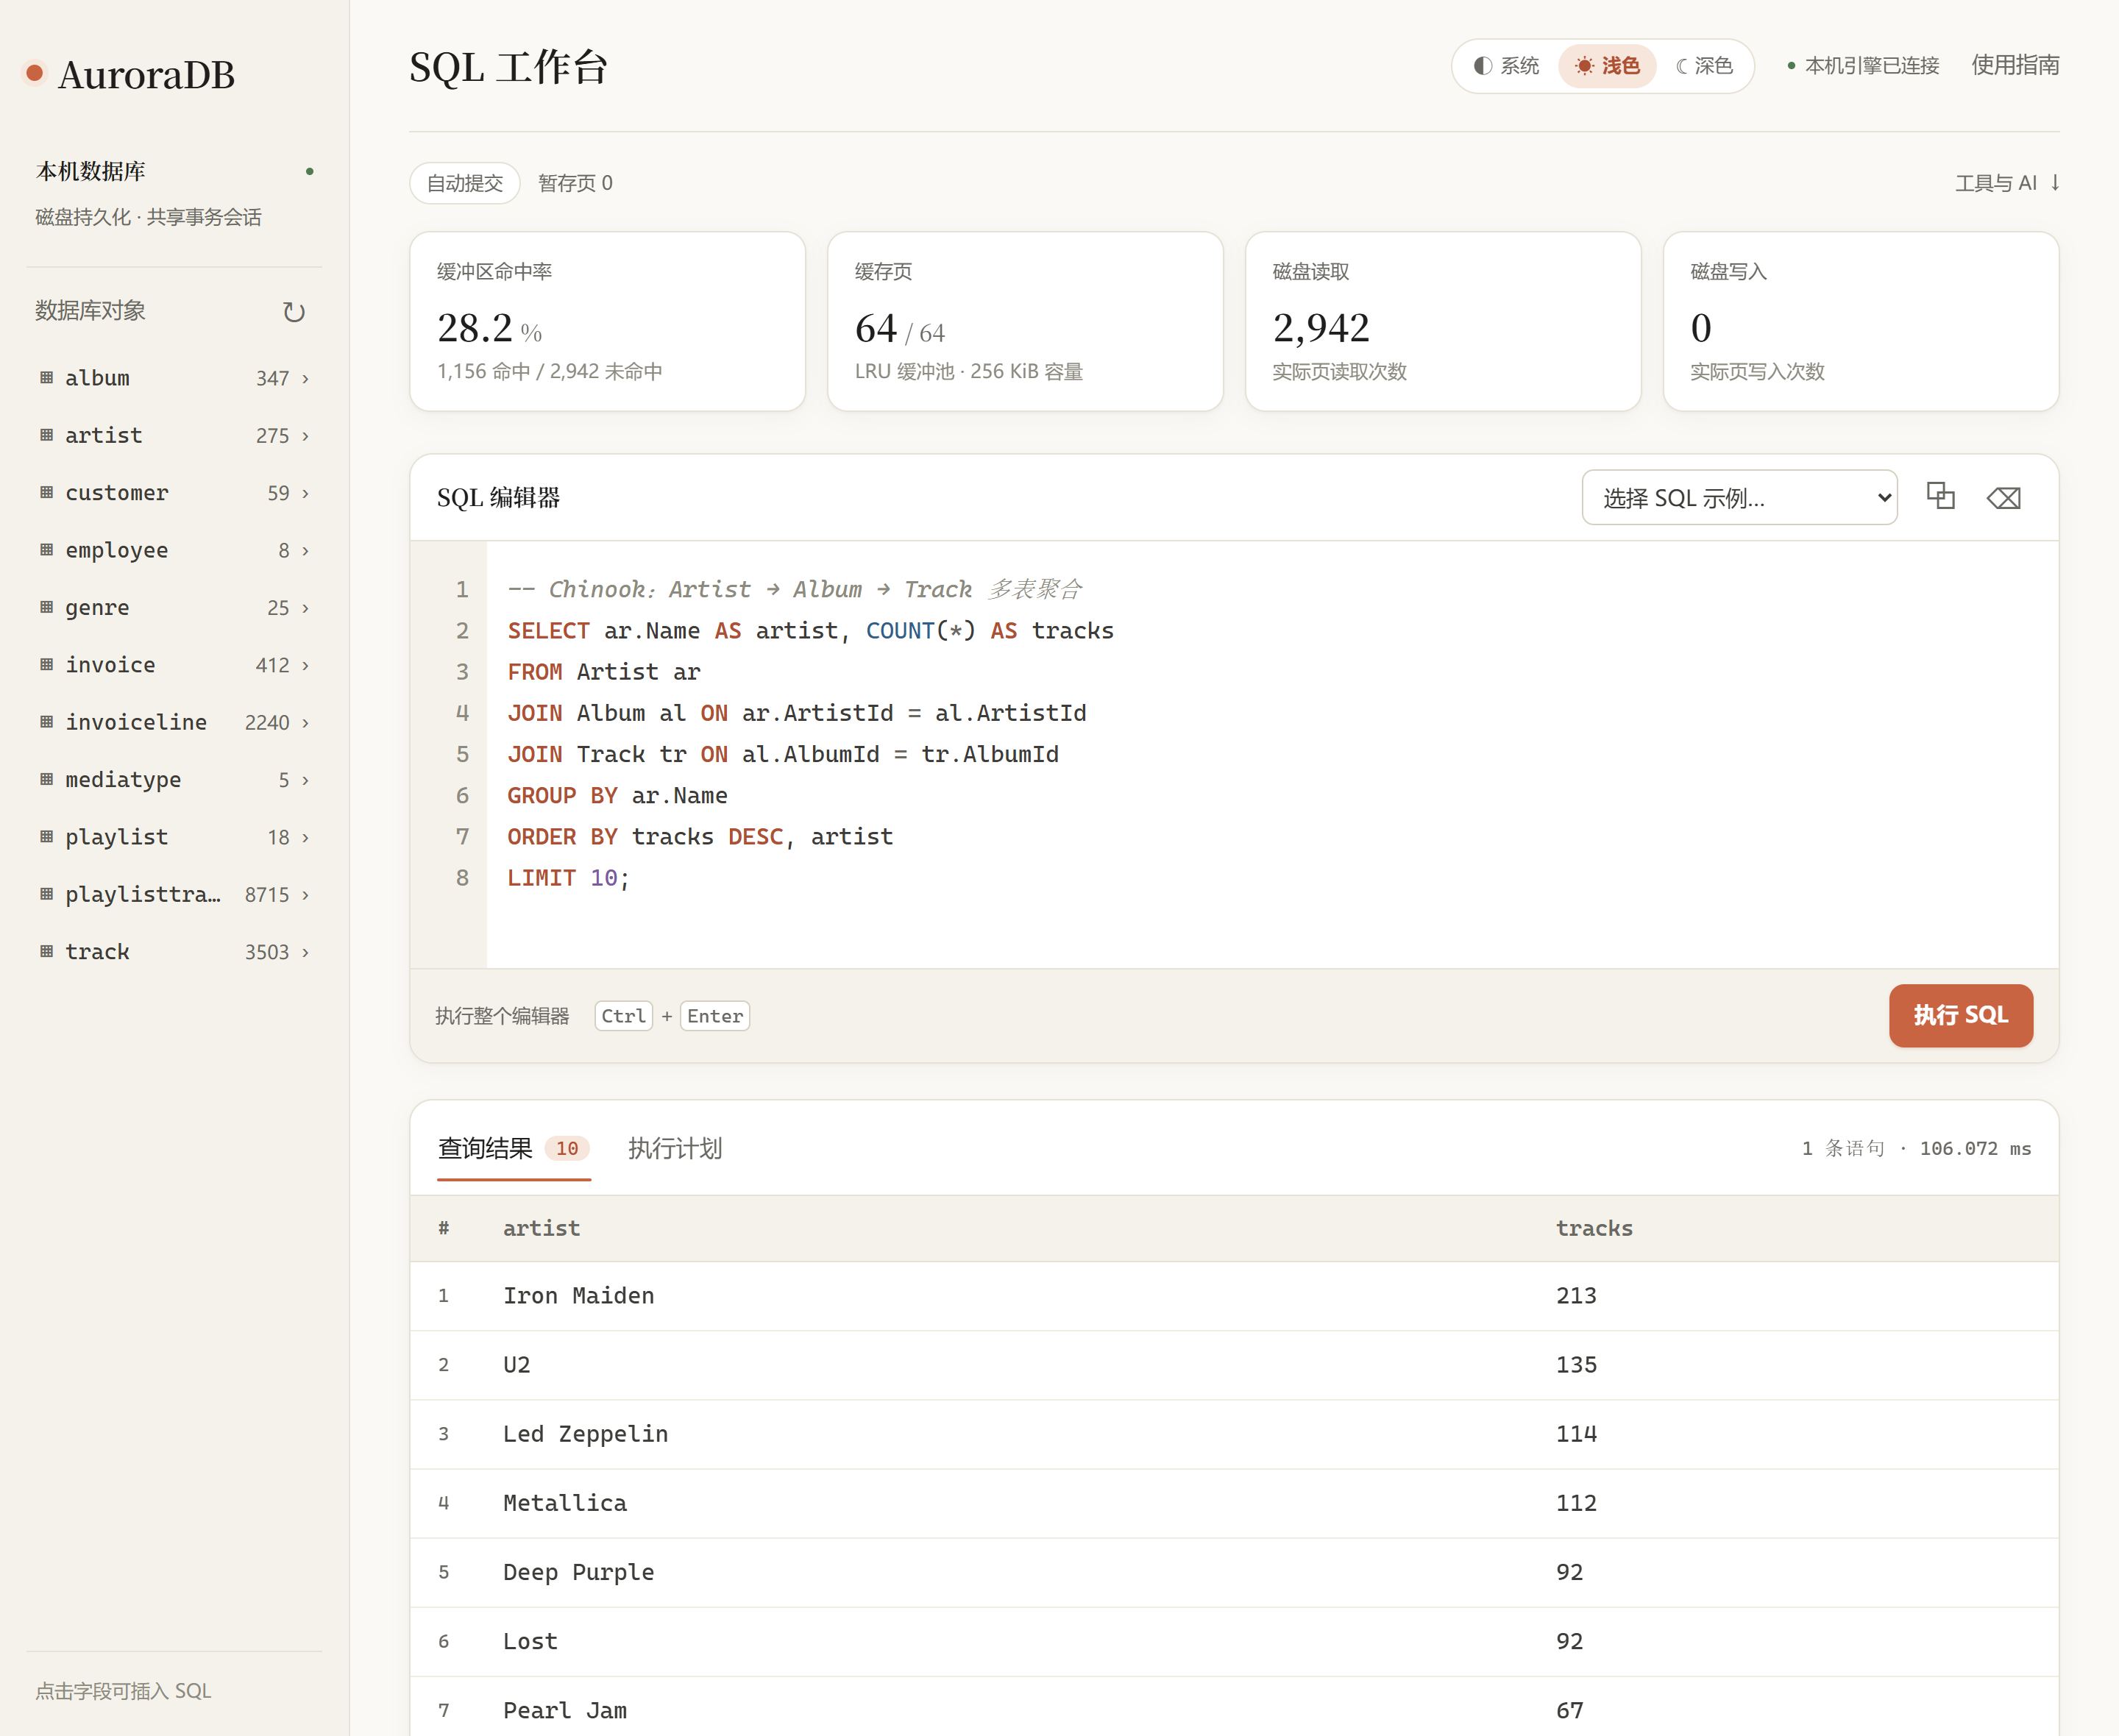
\includegraphics[width=\textwidth]{fig/ui_workbench.png}
\caption{AuroraDB 浏览器工作台（Chinook 数据库，执行“艺术家与曲目 Top 10”示例）}\label{fig:workbench}
\end{figure}

\subsection{命令行界面}
不带 \fn{--web} 参数启动时进入交互式 REPL，支持多行语句、分号结束、\texttt{SHOW TABLES} / \texttt{DESCRIBE} 等诊断命令；
也可以用 \fn{--execute} 执行一段 SQL，或用 \fn{--file} 执行 UTF-8 编码的 SQL 脚本。

\subsection{运行方式}
\paragraph{Windows 可执行程序} 双击仓库根目录下的启动脚本即可：\fn{启动工作台.cmd} 打开中文教学库，
\fn{启动Chinook.cmd} 首次运行时导入 Chinook 数据集（独立目录，不影响教学库）。也可以在命令行中运行：
\begin{lstlisting}[style=py]
dist\AuroraDB.exe --web --demo --db data\aurora
dist\AuroraDB.exe --dataset chinook --web --port 0 --db data\chinook
\end{lstlisting}
\paragraph{源码运行（Windows / macOS / Linux，Python $\ge$ 3.12）}
\begin{lstlisting}[style=py]
python -m auroradb --web --demo                  # web workbench + teaching data
python -m auroradb --dataset chinook --web --db data/chinook
python -m auroradb -e "SELECT * FROM students;"   # one-shot SQL
python -m auroradb                               # interactive REPL
python -m unittest discover -s tests             # run all tests
\end{lstlisting}
\paragraph{AI 功能} 将 \fn{ai.example.json} 复制为 \fn{ai.local.json} 并填入服务地址与密钥后，工作台自动启用 AI 功能；
该文件被 \fn{.gitignore} 排除，打包脚本也会拒绝包含带密钥的配置文件。

\subsection{安全设计}
SQL 只被解析成数据结构，执行器按规则逐个计算，从不调用 \texttt{eval}；语法树深度受限；不支持的语法在出错位置明确报错。
HTTP 服务只监听 127.0.0.1，并校验 Host 头（防止 DNS 重绑定）与 Origin 头（拒绝跨站请求）；
写操作还需携带启动时随机生成的令牌（\texttt{X-Aurora-Token}，用常数时间比较）；请求体必须是不超过 512\,KiB 的 JSON，研究实验另有执行预算。

%==================== 10 测试与实验 ====================
\section{测试与实验}\label{sec:test}

\subsection{测试方法}
测试使用 Python 标准库 \fn{unittest}，分为以下几类：
\begin{itemize}
  \item \textbf{单元测试}：词法、语法、绑定、各算子、页编码、B+ 树分裂与范围扫描、WAL 帧解析等。
  \item \textbf{故障注入与恢复测试}：在提交流程的不同步骤模拟进程崩溃，检查重启后数据与日志的状态；构造损坏的页和日志，
        检查系统报错而不是静默接受。
  \item \textbf{差分测试}：以固定种子 20261009 随机生成 180 条 SELECT，分别在 AuroraDB 与 SQLite 上执行，按多重集合比较结果；
        连接扩展另有 120 条随机查询，在 heuristic 与 adaptive 两种模式下都与 SQLite 核对。
  \item \textbf{集成测试}：真实 HTTP 请求下的工作台接口、Host / Origin / 令牌校验、错误隔离与并发查询；可执行程序的冒烟测试。
  \item \textbf{研究扩展测试}：可信改写的正例与反例、学习模型的就绪与回退、预测缓冲的结果一致性、语义算子的协议校验与预算。
\end{itemize}

\subsection{测试结果}
全部 279 项测试通过（失败 0，错误 0），按子系统的分布见表 \ref{tab:tests}。测试结果由 \fn{tools/verify.py} 生成并写入
\fn{docs/test_results.json}，测试总数不手工填写。

\begin{table}[!htb]
\centering\small
\caption{自动化测试分布（共 279 项，全部通过）}\label{tab:tests}
\begin{tabularx}{\textwidth}{>{\raggedright}p{3.6cm}X>{\raggedleft\arraybackslash}p{1.2cm}}
\toprule
子系统 & 测试文件（测试数） & 合计 \\
\midrule
存储与缓冲 & storage (25)、integrity (20)、predictive\_buffer (12)、integration\_storage (10) & 67 \\
SQL 编译与执行 & sql (23)、regressions (18)、engine (16)、diagnostics (6) & 63 \\
优化：改写 / 学习 / 连接 & research\_optimizer (29)、join\_forms (15)、research\_audit (12)、join\_optimizer (6)、optimizer\_demo (3) & 65 \\
AI 语义、服务与交付 & ai (22)、semantic (17)、server (13)、ai\_deadlines (9)、advanced\_server (9)、ai\_integration (8)、submission (5)、chinook\_dataset (1) & 84 \\
\midrule
合计 & & 279 \\
\bottomrule
\end{tabularx}
\end{table}

测试按层次组织（表 \ref{tab:levels}），从单个函数到真实 HTTP 服务和独立运行的可执行程序。

\begin{table}[H]
\centering\small
\caption{测试层次}\label{tab:levels}
\begin{tabularx}{\textwidth}{>{\raggedright}p{3.0cm}>{\raggedright}X>{\raggedright\arraybackslash}p{4.6cm}}
\toprule
层次 & 内容 & 测试位置 \\
\midrule
\TestLevelRows
\bottomrule
\end{tabularx}
\end{table}

\subsection{测试用例}
表 \ref{tab:tc} 列出 55 个系统测试用例：TC-01 至 TC-53 各对应一个自动化测试方法（报告生成时逐条核对其在
\fn{docs/test_results.json} 中为“通过”），TC-54 与 TC-55 的证据分别是可执行程序冒烟测试和性能基准的记录文件。

{\footnotesize
\begin{longtable}{>{\raggedright}p{0.95cm}>{\raggedright}p{2.3cm}>{\raggedright}p{5.8cm}>{\raggedright}p{3.0cm}>{\raggedright\arraybackslash}p{1.5cm}}
\caption{系统测试用例（全部通过）}\label{tab:tc}\\
\toprule
编号 & 模块 / 测试项 & 输入与预期结果 & 测试文件 & 需求 \\
\midrule
\endfirsthead
\toprule
编号 & 模块 / 测试项 & 输入与预期结果 & 测试文件 & 需求 \\
\midrule
\endhead
\TCRows
\bottomrule
\end{longtable}}

\subsection{需求追踪矩阵}\label{sec:trace}
表 \ref{tab:trace} 把第 \ref{sec:req} 节的每条需求对应到验证它的测试用例，31 条需求均有对应的测试或实验。

{\small
\begin{longtable}{>{\raggedright}p{1.4cm}>{\raggedright}p{4.0cm}>{\raggedright\arraybackslash}p{9.0cm}}
\caption{需求追踪矩阵}\label{tab:trace}\\
\toprule
需求 & 名称 & 验证用例 \\
\midrule
\endfirsthead
\toprule
需求 & 名称 & 验证用例 \\
\midrule
\endhead
\TraceRows
\bottomrule
\end{longtable}}

\subsection{已知缺陷}
测试与评审中发现、但本版本没有修复的问题列于表 \ref{tab:defects}，其中的数据为小组在开发时的实测记录。

\begin{table}[H]
\centering\small
\caption{已知缺陷与改进方向}\label{tab:defects}
\begin{tabularx}{\textwidth}{>{\raggedright}p{1.2cm}>{\raggedright}p{1.1cm}>{\raggedright}X>{\raggedright}p{3.2cm}>{\raggedright\arraybackslash}p{3.0cm}}
\toprule
编号 & 级别 & 问题 & 证据 & 改进方向 \\
\midrule
\DefectRows
\bottomrule
\end{tabularx}
\end{table}

\subsection{实验设置}
所有实验脚本在临时数据库中运行，使用固定的数据生成方式与随机种子，把参数、时间、原始计数和源码 SHA-256 写入 JSON，
源码变化后旧的实验证据会被判定为过期。“读页”指数据库文件的应用层页读取次数，操作系统文件缓存保留；
耗时为包含 Python 开销的墙钟时间，只用于同一批次内的相对比较。

\subsection{可信改写}
实验在 5\,000 行、16 页缓存的数据库上构造 13 个案例（\fn{docs/optimizer_research.json}），全部符合预期，代表性案例见表 \ref{tab:opt}。
在 OR→IN 正例中，扫描行数由 5\,000 降为 2，读页由 109 降为 3，中位耗时由 70.05 ms 降为 1.90 ms。
“短查询回退”案例虽为 proven，但原查询只需 0.04 ms，未达到 2 ms 门槛，因此不建议替换；
未知外部候选即使结果一致也只得到 tested；插入数据后的反例、布尔与数值混淆、外连接与重复行变化都被判为 unknown 并拒绝。

\begin{table}[!htb]
\centering\small
\caption{可信改写实验的代表性案例}\label{tab:opt}
\begin{tabular}{lccc}
\toprule
案例 & 验证级别 & 结果一致 & 建议替换 \\
\midrule
OR→IN 索引改写 & proven & 是 & 是 \\
NULL 与重复 AND 删除 & proven & 是 & 是 \\
排序同值组比较 & proven & 是 & 是 \\
左连接可空列上的 OR & proven & 是 & 否（不够快） \\
短查询回退 & proven & 是 & 否（原查询 $<$ 2 ms） \\
未知外部候选（仅当前数据一致） & tested & 是 & 否 \\
插入数据后的反例 & unknown & 否 & 否 \\
布尔 / 数值混淆反例 & unknown & 否 & 否 \\
外连接反例 & unknown & 否 & 否 \\
\bottomrule
\end{tabular}
\end{table}

\subsection{学习型优化}
36 条训练查询、9 条不参与训练的留出查询，每种模式每条执行 3 次（表 \ref{tab:learn}）。
平滑 Q-error 定义为 $\max\bigl(\tfrac{a+1}{e+1}, \tfrac{e+1}{a+1}\bigr)$，$a$、$e$ 分别为实际与估计行数。
自适应模式下估计误差显著下降，访问路径改变 5 次，没有出现超过 15\% 且 1 ms 的退化，全部结果一致；
P95 耗时基本持平，说明更准确的估计并不必然带来所有查询的加速。阈值单调性检查 101 个点，违规 0 次。

\begin{table}[!htb]
\centering\small
\caption{学习型优化的留出评估（9 条查询）}\label{tab:learn}
\begin{tabular}{lrr}
\toprule
指标 & heuristic & adaptive \\
\midrule
平滑 Q-error 中位数 & 1.850 & 1.027 \\
平滑 Q-error P95 & 2.624 & 1.182 \\
9 条查询中位耗时之和 (ms) & 1342.9 & 847.6 \\
逐查询中位耗时的中位数 (ms) & 147.5 & 68.6 \\
逐查询中位耗时的 P95 (ms) & 253.1 & 255.8 \\
\bottomrule
\end{tabular}
\end{table}

连接扩展方面，三表演示用例的连接候选比较由 20\,000 次降为 200 次（图 \ref{fig:join}）；
100$\times$100 行的范围连接测试中，需要检查完整 ON 条件的候选由 10\,000 次降为 4\,950 次，结果一致。
该计数不含排序与二分的内部比较，不能直接等同于耗时改善比例。

\subsection{预测缓冲}\label{sec:exp-buffer}
6\,000 行数据，四类负载（热点点读夹大扫描、重复范围查询、热点迁移、纯扫描），缓存 8 / 24 / 64 页，采样 1 / 4 / 8 / 32，
每种配置 3 轮并随机化顺序，共 180 次运行、48 组对照，所有查询结果与基准一致。
表 \ref{tab:buffer} 与图 \ref{fig:bufchart} 给出采样数为 8 时与同版 LRU 的对比（Linux 环境，2026-10-28 加入扫描准入后的版本）。

\begin{table}[!htb]
\centering\small
\caption{预测策略与同版 LRU 的对比（采样 8；耗时比 = 预测 / LRU，小于 1 表示更快）}\label{tab:buffer}
\begin{tabular}{lrrrrr}
\toprule
负载 & 缓存页 & LRU 读页 & 预测读页 & 读页减少 & 耗时比 \\
\midrule
\multirow{3}{*}{热点 + 大扫描} & 8 & 4011 & 3989 & 0.55\% & 0.962 \\
 & 24 & 3769 & 3584 & 4.91\% & 0.747 \\
 & 64 & 3769 & 3288 & 12.76\% & 0.765 \\
\midrule
\multirow{3}{*}{重复范围} & 8 & 2496 & 2496 & 0.00\% & 0.995 \\
 & 24 & 2496 & 2496 & 0.00\% & 0.978 \\
 & 64 & 2496 & 2496 & 0.00\% & 0.985 \\
\midrule
\multirow{3}{*}{热点迁移} & 8 & 7497 & 7481 & 0.21\% & 0.951 \\
 & 24 & 7493 & 7136 & 4.76\% & 0.735 \\
 & 64 & 7493 & 6804 & 9.20\% & 0.761 \\
\midrule
\multirow{3}{*}{纯扫描} & 8 & 3696 & 3696 & 0.00\% & 1.129 \\
 & 24 & 3696 & 3696 & 0.00\% & 1.114 \\
 & 64 & 3696 & 3696 & 0.00\% & 1.140 \\
\bottomrule
\end{tabular}
\end{table}

\begin{figure}[!htb]
\centering
\begin{tikzpicture}
\begin{axis}[
  ybar, bar width=7pt, width=0.92\textwidth, height=5.4cm,
  symbolic x coords={热点+大扫描,重复范围,热点迁移,纯扫描},
  xtick=data, ymin=0, ymax=14.5, ylabel={读页减少（\%）},
  legend style={at={(0.5,-0.16)},anchor=north,font=\small,draw=none},
  legend columns=3, tick label style={font=\small}, label style={font=\small},
  nodes near coords, every node near coord/.append style={font=\scriptsize, /pgf/number format/fixed, /pgf/number format/precision=2},
  enlarge x limits=0.18, ymajorgrids, grid style={black!10}]
\addplot[fill=accent!35, draw=accent] coordinates {(热点+大扫描,0.55) (重复范围,0) (热点迁移,0.21) (纯扫描,0)};
\addplot[fill=accent!70, draw=accent] coordinates {(热点+大扫描,4.91) (重复范围,0) (热点迁移,4.76) (纯扫描,0)};
\addplot[fill=warm!80, draw=warm] coordinates {(热点+大扫描,12.76) (重复范围,0) (热点迁移,9.20) (纯扫描,0)};
\legend{8 页,24 页,64 页}
\end{axis}
\end{tikzpicture}
\caption{预测策略相对 LRU 的文件读页减少比例（采样 8）}\label{fig:bufchart}
\end{figure}

在预先选定的“热点 + 大扫描、24 页、采样 8”配置上，预测策略的平均总耗时由 320.8 ms 降为 239.6 ms（降低 25.3\%），
文件读页减少 4.91\%，独立的同场五轮复测降低 23.7\%。耗时改善同时来自读页减少和避免不必要的页对象复制，
不能全部归因于磁盘 I/O。重复范围查询没有读页收益，纯扫描负载下预测策略慢 11\%--14\%，因此它不是普遍更优的策略，
默认仍使用 LRU。

\subsection{语义算子的批处理与缓存}
输入 64 行、完整文本去重后 32 条，使用确定性的本机模拟服务（每次请求人为等待 3 ms）对比三种方式（表 \ref{tab:sem}）。
调用次数的下降来自同次运行内去重、批处理和跨运行的精确缓存，三种方式的结果与预先定义的期望完全一致。
由于使用的是模拟服务，这里的耗时不代表真实大模型的性能，也不评估模型判断的语义质量。

\begin{table}[!htb]
\centering\small
\caption{语义管线的调用次数与耗时（模拟服务）}\label{tab:sem}
\begin{tabular}{lrrrr}
\toprule
方式 & 批大小 & HTTP 调用 & 缓存命中 & 总耗时 (ms) \\
\midrule
逐条调用 & 1 & 32 & 0 & 213.4 \\
批量（冷缓存） & 8 & 4 & 0 & 45.6 \\
批量（热缓存） & 8 & 0 & 32 & 1.4 \\
\bottomrule
\end{tabular}
\end{table}

\subsection{公开数据集}
Chinook \cite{chinook} 是一个以音乐商店为背景的公开示例数据库（MIT 许可）。导入器 \fn{tools/import_chinook.py}
把其中 AuroraDB 支持的列类型映射为 INTEGER、REAL、TEXT、BOOLEAN，跳过视图、触发器与二进制列，
共导入 11 张表、15\,607 行（Track 3\,503、PlaylistTrack 8\,715、InvoiceLine 2\,240 等），每张表的预期行数由测试核对。
Chinook 用于展示多表连接、聚合和索引计划；定量的性能结论仍以固定种子的受控实验为准。

\subsection{有效性威胁}
有限的 SQL 子集、单连接串行执行和小规模合成负载限制了结论的外部有效性；有限数据上的结果比较不能证明任意数据库上的等价；
墙钟耗时受 CPU 调度和宿主机负载影响，跨批次的数字不能直接比较；文献中的性能结果只用于介绍方法，不作为本项目的结论。

%==================== 项目管理 ====================
\section{项目管理与配置管理}\label{sec:pm}

\subsection{开发过程模型}
项目采用迭代增量模型：先完成可以独立测试的存储内核，再逐层向上实现 SQL 编译、执行与界面，最后加入研究扩展。
每个迭代以对应的自动化测试全部通过作为完成标准（表 \ref{tab:iter}）。

\begin{table}[H]
\centering\small
\caption{迭代计划}\label{tab:iter}
\begin{tabularx}{\textwidth}{>{\raggedright}p{1.3cm}>{\raggedright}p{2.8cm}>{\raggedright}X>{\raggedright\arraybackslash}p{4.4cm}}
\toprule
迭代 & 主题 & 主要产出 & 完成标准 \\
\midrule
\IterRows
\bottomrule
\end{tabularx}
\end{table}

\subsection{配置管理与编码规范}
\begin{itemize}
  \item \textbf{版本控制}：Git，远程仓库 \url{https://github.com/Guopeng-Zhong/AuroraDB}，主分支 main。
  \item \textbf{版本号}：\fn{pyproject.toml} 与 \fn{auroradb/__init__.py} 统一维护，当前为 1.2.0。
  \item \textbf{忽略规则}：\fn{.gitignore} 排除数据库文件、日志、构建目录与 \fn{*.local.json} 私有配置。
  \item \textbf{回归}：每次提交前运行 \fn{python tools/verify.py}，全部测试通过才合并；结果写入 \fn{docs/test_results.json}。
  \item \textbf{构建与交付}：\fn{python tools/build_exe.py} 生成 \fn{dist/AuroraDB.exe}；
        \fn{python tools/package_submission.py} 生成提交包，并用 \fn{MANIFEST.json} 记录每个文件的 SHA-256。
  \item \textbf{编码规范}：每个源文件以文档字符串说明职责、边界与不变量；用户可见错误统一为 \fn{DatabaseError}，
        存储层错误为 \fn{StorageError}；测试方法命名为 \fn{test_<被验证的行为>}，一个方法验证一个行为；
        运行时只使用 Python 标准库，文档与打包工具的依赖不进入运行时。
\end{itemize}

%==================== 11 分工 ====================
\section{小组分工与完成情况}\label{sec:team}

小组共四人，按“一个人负责一个子系统和一个对应创新点”的方式分工；需求分析、总体架构讨论、接口联调、
代码与结果核验、测试复现、报告撰写和答辩准备由四人共同参与。模块负责人承担该部分的设计、实现组织与核验责任。
经小组确认，四人工作量占比各为 25\%。

\begin{table}[!htb]
\centering\small
\caption{小组分工与完成情况}\label{tab:team}
\begin{tabularx}{\textwidth}{>{\raggedright}p{1.6cm}>{\raggedright}p{2.6cm}>{\raggedright}X>{\raggedright\arraybackslash}p{3.0cm}}
\toprule
成员 & 角色 & 负责内容 & 主要源文件 / 测试 \\
\midrule
钟国鹏 & SQL 编译与可信查询执行 &
SQL 词法 / 语法分析、名称绑定、访问路径选择；扫描、连接、聚合与事务执行；
创新点为可信查询改写（规则证据、结果核验、收益门槛与保守推荐）；工作台中 SQL 编辑器、执行计划、扫描对比与可信改写面板；小组协调与汇报整合 &
\fn{sql.py} \fn{engine.py} \fn{optimizer.py}；test\_sql、test\_engine、test\_regressions、test\_diagnostics、test\_research\_optimizer \\
\midrule
曾子恒 & 数据存储与预测缓冲 &
页格式与 CRC、堆表、B+ 树、WAL 与崩溃恢复、一致性检查；LRU 缓冲与扫描感知预测淘汰、扫描准入与页对象所有权优化；缓冲实验 &
\fn{storage.py} \fn{integrity.py}；test\_storage、test\_integration\_storage、test\_integrity、test\_predictive\_buffer \\
\midrule
黄俊植 & 统计学习与性能优化 &
列统计、轻量基数 / 读成本 / 连接成本模型、有界工作负载反馈、3--6 表内连接动态规划、范围连接与连接规范化、
置信度 / 域外 / 预算回退、执行计划诊断，以及训练 / 留出 / 漂移实验 &
\fn{learning.py} \fn{workload.py} \fn{join_planning.py} \fn{join_optimizer.py}；test\_join\_optimizer、test\_join\_forms、test\_research\_audit \\
\midrule
路茗淳 & AI 语义、交互与交付 &
语义筛选 / 分类 / 聚合算子、批处理与缓存协议、AI 接口与校园模型接入；浏览器工作台框架、命令行、HTTP 安全校验；
打包、测试脚本与文档生成 &
\fn{semantic.py} \fn{ai.py} \fn{server.py} \fn{__main__.py} \fn{web/}；test\_semantic、test\_ai*、test\_server \\
\bottomrule
\end{tabularx}
\end{table}

%==================== 12 局限与展望 ====================
\section{局限与展望}
\begin{itemize}
  \item \textbf{SQL 覆盖}：没有子查询、窗口函数、RIGHT / FULL JOIN、外键、复合索引、ALTER TABLE 与视图。
  \item \textbf{并发}：单写者、单事务设计，没有 MVCC 与并发控制协议；预测缓冲的并发扫描场景未被研究。
  \item \textbf{存储}：JSON 页体可读但空间利用率低；B+ 树删除采用延迟合并，删除大量数据后需要重建；不回收不可达的溢出页与目录分片。
  \item \textbf{可信改写}：目前只有 3 条规则且只改写 WHERE；证明只覆盖本项目实现的 SQL 方言。后续可增加谓词下推、常量折叠等规则，
        并对证明不了的候选引入 SMT 求解或自动反例搜索。
  \item \textbf{学习与 AI}：没有跨数据库预训练与在线漂移理论保证；语义算子的真实模型质量需要更大的人工标注集评估。
\end{itemize}

%==================== 13 结论 ====================
\section{结论}
本组从磁盘页、B+ 树和预写日志出发，自研实现了包含存储管理器、缓冲管理器、查询处理器、执行引擎和用户界面的关系数据库 AuroraDB，
满足课程方案 1 的全部组件要求，并以 279 项自动化测试（含与 SQLite 的差分测试）验证其正确性。
在可观察的内核之上，四位成员分别完成了可信查询改写、统计学习与自适应连接、预测式缓冲和 AI 语义算子四项扩展。
这些扩展有一个共同的设计取向：\textbf{把“看起来更好”与“证明是对的”分开，证据不足时回到确定、保守的路径}。
可信改写只替换经规则证明、全量核验且实测更快的查询；学习模型越界即回退；预测缓冲证据不足即回到 LRU；
AI 算子的输出受协议校验与预算约束。我们认为，这种“可验证的智能优化”是把研究思想落到可运行系统时最重要的工程原则。

%==================== 参考文献 ====================
\clearpage
\begin{thebibliography}{99}
\addcontentsline{toc}{section}{参考文献}
\small
\bibitem{codd1970} Codd E F. A relational model of data for large shared data banks[J]. Communications of the ACM, 1970, 13(6): 377--387.
\bibitem{silberschatz2019} Silberschatz A, Korth H F, Sudarshan S. Database System Concepts[M]. 7th ed. New York: McGraw-Hill, 2019.
\bibitem{gmuw2008} Garcia-Molina H, Ullman J D, Widom J. Database Systems: The Complete Book[M]. 2nd ed. Upper Saddle River: Pearson Prentice Hall, 2008.
\bibitem{bayer1972} Bayer R, McCreight E. Organization and maintenance of large ordered indexes[J]. Acta Informatica, 1972, 1(3): 173--189.
\bibitem{comer1979} Comer D. The ubiquitous B-tree[J]. ACM Computing Surveys, 1979, 11(2): 121--137.
\bibitem{selinger1979} Selinger P G, Astrahan M M, Chamberlin D D, et al. Access path selection in a relational database management system[C]//Proceedings of the 1979 ACM SIGMOD International Conference on Management of Data. 1979: 23--34.
\bibitem{graefe1993} Graefe G. Query evaluation techniques for large databases[J]. ACM Computing Surveys, 1993, 25(2): 73--169.
\bibitem{mohan1992} Mohan C, Haderle D, Lindsay B, et al. ARIES: a transaction recovery method supporting fine-granularity locking and partial rollbacks using write-ahead logging[J]. ACM Transactions on Database Systems, 1992, 17(1): 94--162.
\bibitem{oneil1993} O'Neil E J, O'Neil P E, Weikum G. The LRU-K page replacement algorithm for database disk buffering[C]//Proceedings of the 1993 ACM SIGMOD International Conference on Management of Data. 1993: 297--306.
\bibitem{leis2015} Leis V, Gubichev A, Mirchev A, et al. How good are query optimizers, really?[J]. Proceedings of the VLDB Endowment, 2015, 9(3): 204--215.
\bibitem{chu2017} Chu S, Wang C, Weitz K, et al. Cosette: an automated prover for SQL[C]//Proceedings of the 8th Biennial Conference on Innovative Data Systems Research (CIDR). 2017.
\bibitem{narasayya2026} Narasayya V, Chaudhuri S. Leveraging query optimizers to verify the soundness of LLM-based query rewrites for real-world workloads, and more![C]//Proceedings of the Conference on Innovative Data Systems Research (CIDR). 2026. \url{https://www.vldb.org/cidrdb/papers/2026/p33-narasayya.pdf}.
\bibitem{resequel2026} Fathollahzadeh S, Mansour E, Boehm M. ReSequel: robust LLM-assisted query rewriting and optimization using templatization and sampling[J]. Proceedings of the VLDB Endowment, 2026, 19(10): 2880--2893. DOI: 10.14778/3828612.3828639.
\bibitem{price2024} Zeng T, Lan J, Ma J, et al. PRICE: a pretrained model for cross-database cardinality estimation[J]. Proceedings of the VLDB Endowment, 2024, 18(3): 637--650. DOI: 10.14778/3712221.3712231.
\bibitem{cardood2026} Li R, Zhao K, Yu J X, Wang G. CardOOD: robust query-driven cardinality estimation under out-of-distribution[J]. The VLDB Journal, 2026, 35(4): 28. DOI: 10.1007/s00778-026-00979-3.
\bibitem{khalaji2025} Khalaji M, Vanderkooy T, Guo R B, Daudjee K. Sampling-based predictive database buffer management[J]. Proceedings of the VLDB Endowment, 2025, 18(13): 5569--5581. DOI: 10.14778/3773731.3773734.
\bibitem{ipdb2026} Kumarasinghe U, Liu T, Mahmood A R, Liu C, Aref W G. iPDB: optimizing semantic SQL queries[EB/OL]. arXiv: 2601.16432, 2026. \url{https://arxiv.org/abs/2601.16432}.
\bibitem{chinook} Rocha L. Chinook Database, version 1.4.5[EB/OL]. \url{https://github.com/lerocha/chinook-database}.
\end{thebibliography}

%==================== 附录 ====================
\appendix
\section{复现步骤与仓库结构}
在仓库根目录依次执行以下命令，可重新运行全部测试与实验并生成证据文件：
\begin{lstlisting}[style=py]
python tools/verify.py                  # 279 tests -> docs/test_results.json
python tools/optimizer_experiment.py    # -> docs/optimizer_research.json
python tools/buffer_experiment.py       # -> docs/buffer_research.json
python tools/semantic_experiment.py     # -> docs/semantic_research.json
python tools/join_optimizer_experiment.py
python tools/build_exe.py               # build dist/AuroraDB.exe
python tools/executable_smoke.py        # smoke-test the executable
\end{lstlisting}

\begin{table}[!htb]
\centering\small
\caption{仓库目录结构}
\begin{tabularx}{\textwidth}{>{\ttfamily}p{4.2cm}X}
\toprule
\normalfont 路径 & 内容 \\
\midrule
auroradb/ & 数据库内核、研究扩展、HTTP 服务与前端（\fn{web/}） \\
tests/ & 279 项自动化测试 \\
tools/ & 实验、构建、打包与文档生成脚本 \\
dist/AuroraDB.exe & Windows 单文件可执行程序 \\
docs/ & 本报告、内部设计说明与实验证据 JSON \\
\bottomrule
\end{tabularx}
\end{table}

\end{document}
